%
% ─── CAPITULO 8: INTRODUCCION AL RAY TRACING ────────────────────────────────────
%

En los anteriores capítulos hemos visto cómo asignar colores a los píxeles utilizando el fragment shader y cómo dibujar hermosos fractales en la superficie que ocupan dos triángulos. Sin embargo, no hemos podido movernos de las dos dimensiones. Esto se debe a la dificultad que de por sí supone que en 2D un píxel puede representar un único punto del plano mientras que en 3D un píxel representa infinitos puntos del espacio. Nuestro objetivo ahora es poder visualizar escenas simples en 3D para posteriormente generar fractales tridimensionales. El código del fragment shader que se emplea en este capítulo se puede encontrar en el fichero \verb|static/glsl/fragment-shader-ray-tracer.js|, también disponible en \url{https://github.com/JAntonioVR/Geometria-Fractal/blob/main/static/glsl/fragment-shader-ray-tracer.js}.

\section{Definición de Ray-Tracing}

En el mundo de la informática gráfica existen dos formas fundamentales de proceder a la representación de escenas. Supongamos que tenemos una escena 3D con varios objetos, como pueden ser por ejemplo un cubo y un par de esferas y queremos visualizar la misma en un canvas 2D.
\begin{itemize}
    \item Una de las formas de representarla es la \textbf{rasterización}, ya introducida al inicio del capítulo \ref{chap:visualizacion}. Esta técnica se basa en modelos de fronteras de objetos 3D. Esto es, se representan objetos constituidos a partir de conjuntos de caras planas poligonales (típicamente triángulos), y se denominan primitivas a dichas caras. Pensemos por ejemplo en un cono como una pirámide cuya base es un polígono regular de muchos lados. El método consiste en identificar para cada primitiva que compone la escena qué píxeles ocupa y asignar color a cada píxel, aplicando posibles modelos de iluminación y texturas.
    \item Otra forma es, para cada pixel, calcular qué primitivas de la escena se proyectan sobre dicho píxel y colorearlo dependiendo de la primitiva más cercana al observador. Esta es la base del \textbf{Ray-Tracing}. En este caso los objetos son representados mediante un algoritmo de cálculo de intersección entre una semirrecta (rayo) y la superficie del objeto en cuestión. Esto engloba los modelos de fronteras utilizados en rasterización, pero además abre posibilidades como objetos con extensión infinita o los propios fractales, que son nuestro principal objetivo.
\end{itemize}

Más en profundidad, la idea es situar al observador en una cierta posición de la escena y colocar frente a él un plano, que llamaremos \textit{plano de proyección}, el cual estará dividido en tantos píxeles como tenga el canvas, de tal manera que se `trazan rayos' que salen desde la posición del observador (en adelante también llamada `punto de vista' o `foco de la proyección') en dirección a cada píxel, por lo que se lanzan tantos rayos como píxeles haya. El rayo atraviesa el plano y avanza por la escena hasta que encuentra la intersección con un objeto. En este caso, se calcula en qué punto se ha alcanzado la intersección y se evalúa un modelo de iluminación o se asigna un color dependiendo de las características de la escena. También es posible que el rayo no alcance ningún objeto, en cuyo caso habría que saber qué hacer con los píxeles cuyos rayos se pierden en el infinito. En la imagen \ref{fig:RT} se puede observar un esquema aclarativo del funcionamiento de este método.

\begin{figure} [ht]
    \centering
    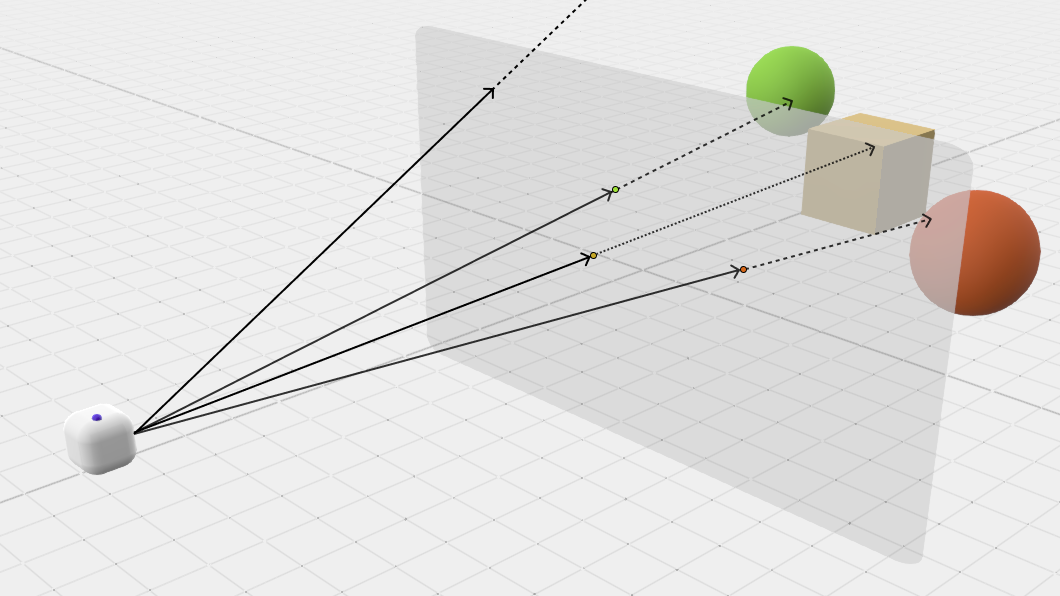
\includegraphics[width=9cm]{img/C8/RT.png}
    \caption{Esquema básico del funcionamiento del Ray-Tracing}
    \label{fig:RT}
\end{figure}

La principal ventaja que tiene el Ray-Tracing (en adelante RT) sobre la rasterización es que este trazado de rayos nos permite facilitar el cálculo de los reflejos y sombras creados por las iluminaciones del entorno, consiguiendo así efectos mucho más realistas en las escenas. Además, las figuras fractales como objetos matemáticos ideales carecen de una superficie o frontera que sea una variedad bidimensional o superficie regular continua, ni siquiera continua a trozos, por lo que no es posible representarlos idealmente utilizando modelos de fronteras como los que utiliza la rasterización. 

No obstante, al igual que en la mayoría de problemas de computación gráfica, los fractales 3D se pueden convertir a modelos de fronteras asumiendo un cierto error de discretización, el cual es totalmente inevitable. Por tanto, partiendo de este hecho, es posible visualizar esos modelos con rasterización o con ray-tracing. Sin embargo, esa conversión es lenta y produce modelos de gran tamaño en memoria. 

Por tanto, es mucho más sencillo usar RT, el cual, si bien también es algo aproximado, es muchísimo más eficiente en memoria, ya que no requiere de ninguna estructura de datos, sino simplemente de un algoritmo de intersección aproximado entre una semirrecta y el fractal. Además no emplea tiempo en la conversión a modelo de fronteras. 

Otra gran ventaja del ray-tracing sobre la rasterización es la dificultad de elegir una conversión a modelos de fronteras con una resolución adecuada. Si la discretización es demasiado fina el tiempo de computación crece mientras que se consigue una mayor resolución, y si no es lo suficientemente fina se pierde mucha resolución.

Sin embargo, este algoritmo tiene una principal desventaja, y es que es un proceso muy costoso, y más aún cuanto más detalle queramos conseguir. Es por esto que ha sido muy difícil dar el salto al ray tracing en tiempo real. Por ejemplo, en el mundo de los videojuegos NVIDIA, que es una famosa empresa desarrolladora de GPUs, comenzó a desarrollar algoritmos para poder utilizar RT en sus GPUs hace varios años, pero hasta finales de 2018 no salieron al mercado las primeras gráficas con estas características. Por su parte, los juegos también deben soportar el algoritmo, por lo que aún son una minoría de videojuegos los que en la actualidad soportan Ray Tracing. En un futuro no muy lejano es posible que haya una tendencia a un desarrollo masivo de juegos que utilicen RT, pero de momento solo tenemos algunos ejemplos como Battlefield V, Minecraft, Metro Exodus, Watch Dogs y Call of Duty: Modern Warfare (2019).

En resumen, y por todas las ventajas y a pesar de las desventajas que hemos descrito de RT sobre la rasterización y los modelos de fronteras en nuestro problema concreto, tomamos la decisión de programar un \textit{ray-tracer} inicialmente básico con el objetivo futuro de generar fractales 3D. La idea por tanto es lanzar rayos a cada píxel y en caso de encontrar intersección con el objeto evaluar un modelo de iluminación para asignar un color concreto.

\section{Elementos y estructura de un Ray-Tracer}
\label{section:elementos-RT}

Hasta ahora hemos visto y explicado en qué consiste el algoritmo RT desde un punto de vista básico. Veamos ahora qué componentes tiene un programa que emplee ray-tracing y conceptos generales, pero más concretos, acerca del cálculo de intersecciones entre semirrectas y objetos 3D. Tres de los componentes más esenciales en un \textit{ray-tracer} son:

\begin{itemize}
    \item \textbf{Generación de rayos primarios}: Por cada píxel se crea un rayo (llamado \textit{rayo primario} o \textit{rayo de cámara}).
    \item \textbf{Cálculo de intersecciones}: Dado un punto $o\in\R^3$ y un vector $\vec v\in\R^3$, se trata de encontrar, si existe, el mínimo valor positivo de $t$ tal que el punto $p(t)=o+\vec v t$ se encuentra en la superficie o frontera de algún objeto de la escena.
    \item \textbf{Modelo de Iluminación Local}: Abreviado como MIL, calcula el color que se asigna a cada píxel cuyo rayo asociado ha intersecado un objeto en función del material asignado, las fuentes de luz y el punto de intersección rayo-objeto. RT además en este caso nos proporciona una poderosa ventaja, pues trazando un rayo desde cualquier punto de la escena en dirección a una fuente de luz podemos conocer si dicho punto está o no en la sombra arrojada de algún objeto sin más que evaluar si el rayo encuentra alguna intersección en su camino hacia la fuente de luz.
\end{itemize}

Con estos tres elementos, una primera descripción en pseudocódigo del algoritmo fundamental de Ray-Tracing sería el del algoritmo \ref{alg:Ray-Tracing}.

\begin{algorithm}[!]
    \caption{Ray Tracing} \label{alg:Ray-Tracing}
    \begin{algorithmic}
        \State $o\gets$ posición del observador en WC.
        \For{cada píxel $(i,j)$ del canvas}
            \State $q\gets$punto central del píxel $(i,j)$ en WC
            \State $\vec v\gets$ vector desde $o$ hasta $q$
            \State $O\gets$ primer objeto visible desde $o$ en la dirección $\vec v$
            \If{no existe objeto visible}
                \State $rad\gets$ color de fondo para $\vec v$ 
            \Else
                \State $p\gets$ punto de intersección en $O$
                \State $rad\gets$ evaluarMIL($O,p$).
            \EndIf
            \State Asignar el color $rad$ al píxel $(i,j)$
        \EndFor
    \end{algorithmic}
\end{algorithm}

Sobre el cálculo de intersecciones, en caso de que se utilicen modelos de fronteras es necesario a su vez utilizar indexación espacial. Esto es, dividir jerárquicamente el espacio en zonas de forma que sea más sencillo localizar un objeto. Esto se debe a que, en caso de encontrarse una intersección con un objeto, para saber de cual se trata podemos hacer una búsqueda secuencial, pero sería muy ineficiente en escenas muy complejas. Por ello, se divide en regiones el espacio y se busca en orden de complejidad logarítmica.

Por su parte, para intersecciones de rayos con objetos no definidos mediante modelos de fronteras debemos calcular el primer cero de determinado campo escalar a lo largo del rayo. Para ello hay dos posibilidades:
\begin{itemize}
    \item \textbf{Usando expresiones analíticas}. Por ejemplo, una esfera de centro $c\in\R^3$ y radio $r>0$ encuentra una intersección con el rayo $o+\vec v t$ en el punto que se verifica la ecuación
    $$
    \|o+\vec v t - c\| - r = 0
    $$
    Este tema se aborda con detalle en la sección \ref{subsection:esfera}.
    \item \textbf{Con un método iterativo}. En ocasiones la resolución de estas ecuaciones es demasiado compleja, por lo que se abordan soluciones iterativas, como pueden ser técnicas estándar de resolución de ecuaciones como el método de Newton. Dentro de esta posibilidad, podemos también contar con una función que estima la distancia a la superficie del objeto y aplicar el algoritmo conocido como `ray marching' o `sphere tracing', el cual explicaremos detenidamente en la sección \ref{section:sphere-tracing}, pero adelantamos que fue introducido por Hart en \cite{Hart-1995}.
\end{itemize}


A partir de ahora, veremos como implementar un \textit{ray-tracer} básico utilizando WebGL. Utilizaremos objetos sencillos como planos y esferas, cuyas intersecciones con rayos se pueden calcular fácilmente de forma analítica sin recurrir a métodos iterativos ni a modelos de fronteras.

En nuestro caso, y de manera similar a la efectuada con los fractales 2D, el vertex shader utilizado es trivial, de hecho es exactamente el mismo que se puede encontrar al inicio del capítulo \ref{chap:fractales-2D}. Por tanto el grueso de la programación se hará de nuevo en el fragment shader, que es el que se ejecuta una vez por píxel. Por su parte, usaremos JavaScript para pasarle variables uniform al shader y para añadir interactividad a la escena. Usaremos de nuevo las clases \verb|Shader| y \verb|Buffer|, pero por las diferencias que existen entre los parámetros de una escena en 2D y una escena en 3D se ha implementado una nueva clase \verb|Scene3D|, que realmente hace lo mismo que \verb|Scene2D| pero utilizando parámetros que requiere una escena 3D. También para gestionar la interacción usuario-escena se ha utilizado un nuevo fichero de JavaScript: \verb|fractals-3D.js|, llamado así porque es el mismo fichero que en el futuro utilizaremos para interactuar con fractales. Recomendamos revisitar la sección \ref{section:codigo} para recordar el papel que realiza la escena y el fichero que gestiona la interacción y los eventos. Puede consultar la documentación del código de JavaScript en el apéndice \ref{appendix:javascript}.

Las siguientes secciones irán dedicadas a explicar la programación del fragment shader, ya que es el elemento que mayor complejidad y lógica contiene.

\section{Creación de rayos primarios}
\label{section:rayo}

Recordamos que cuando se trataba de fractales 2D utilizamos una transformación afín para identificar cada píxel con un punto del plano complejo (sección \ref{section:pantalla-plano}). En este caso debemos identificar cada píxel con un punto no del plano complejo, sino del \textit{plano de proyección} ($P$), que es el plano que colocamos frente al espectador dividido en tantos píxeles como tenga el canvas, de forma que se trazan rayos desde el espectador y hacia dichos píxeles. Supongamos a partir de ahora que queremos representar la escena en un canvas de $n_x\times n_y$ píxeles.

Para cada píxel debemos calcular su posición central en coordenadas de mundo a partir de las coordenadas de dispositivo, que son dos valores enteros $(x',y')$, aunque para identificar cada píxel con su centro tomaremos como coordenadas de dispositivo $(x,y)=(x',y')+\left(\frac 1 2, \frac 1 2\right)$. Este proceso es justamente el contrario al que se utiliza en rasterización, donde se necesita convertir las coordenadas de mundo de las primitivas en coordenadas de dispositivo. Para ello, se utiliza una matriz $M$ que es la composición de la matriz de vista 3D, la cual transforma coordenadas de mundo (WC) a coordenadas de cámara junto con la matriz de proyección, que calcula las coordenadas de dispositivo (DC) a partir de las coordenadas de cámara (véase la analogía con los párrafos que describen la transformación \ref{eq:transformacion-lineal-matrix}). Por tanto, en cierto sentido lo que buscamos es buscar una transformación afín asociada a la inversa de la matriz $M$.

En nuestro caso concreto, y al igual que en el caso 2-dimensional, utilizaremos un canvas de $1280\times 720$ píxeles, que guarda una proporción de $16:9$.

\begin{lstlisting}
<canvas id="glCanvas" width="1280" height="720"></canvas>
\end{lstlisting}

Inicialmente, supongamos que el observador se sitúa en el punto $(0,0,0)$ y que el plano de proyección se sitúa a distancia 1 en el eje negativo $Z$. Esta distancia del observador al plano de proyección es la conocida como la \textit{distancia focal}. Se denomina \textit{lookfrom} u origen y denotamos como $o_c$ al punto desde el que se observa, es decir, en el que se sitúa el observador; y \textit{lookat} o punto de atención $a_t$ al punto hacia el que mira, que en este caso sería el $(0,0,-1)$. En ocasiones nos referiremos al punto $o_c$ como posición del observador o punto de vista.

Como convención asumimos que a la derecha se sitúa el eje positivo $X$, hacia arriba el eje positivo $Y$ y el `interior de la pantalla' es el eje negativo $Z$. Asumimos ahora también que el plano de proyección tiene 2 unidades de alto, lo cual implica que si el ratio ancho/alto es $16/9$ entonces el ancho es de $3.55$ unidades, aunque ese es un valor que calcularemos y almacenaremos en una variable y no importará realmente cual sea.

Un rayo es en realidad simplemente una semirrecta de $\R^3$, las cuales están unívocamente determinadas por un punto $p$ del espacio afín $\R^3$ al cual llamaremos \textit{origen} y por un vector $\vec v$ del espacio vectorial $\R^3$ que denominamos \textit{dirección}. De esta forma, un rayo puede ser expresado como la imagen de la función

$$
R(t) = p + t\cdot \vec v \ \ \forall t\in\R_0^+,
$$
de forma que para cualquier punto $p_0$ del rayo $R$ existe un único $t_0\in\R_0^+$ tal que $R(t_0) = p_0$.

A nivel de código GLSL, la manera de representar un rayo será utilizando una estructura (\verb|struct|) que denominaremos \verb|Ray|. Las estructuras en GLSL son muy parecidas en sintaxis y también en uso a las del lenguaje C. 

\begin{lstlisting}
struct Ray {
    vec3 orig;      // Origen del rayo
    vec3 dir;       // Direccion del rayo
};
\end{lstlisting}

Y si dado un rayo $R$ queremos calcular qué punto de $\R^3$ le corresponde a cierto $t\in\R_0^+$, utilizamos la siguiente función.

\begin{lstlisting}
vec3 ray_at(Ray R, float t){
    return R.orig + t*R.dir;
}
\end{lstlisting}

Esta función nos será útil a la hora de calcular el punto exacto en el que se produce una intersección rayo-objeto cuando solo se conoce la distancia $t$ a la que se produce el impacto.

\begin{observacion}
    Realmente se pueden utilizar valores de $t\in\R$ positivos o negativos, pero pensemos que los valores negativos corresponden a puntos del rayo situados detrás del observador, que no se pueden ver, por lo que es preferible restringirnos a valores no negativos.
\end{observacion}

Una vez tenemos determinada una forma de representar un rayo, es momento de crear uno cuyo origen sea la posición del observador y su dirección sea el vector que tiene como origen el observador y como destino el punto del plano de proyección que identificamos con el píxel. En la situación hipotética que hemos planteado antes en la cual $o_c=(0,0,0)$, llamamos $d_f$ a la distancia focal, $P_h=2$ a la altura del plano de proyección, $P_w$ a la anchura del plano de proyección, $r = 16/9$ (\textit{aspect ratio}) a la proporción $r = \frac{P_w}{P_h}$, de forma que se verifica $P_w=r\cdot P_h$. Con estas variables, llamemos $\mathrm{LLC}$ (\textit{Lower Left Corner}) al punto situado en la esquina inferior izquierda del plano de proyección, entonces:
\begin{equation}
    \label{eq:LLC-inicial}
    \mathrm{LLC} = o_c - \frac{P_w}{2}\cdot(1,0,0) - \frac{P_h}{2}\cdot(0,1,0) - d_f \cdot (0,0,1)
\end{equation}

\begin{figure} [ht]
    \centering
    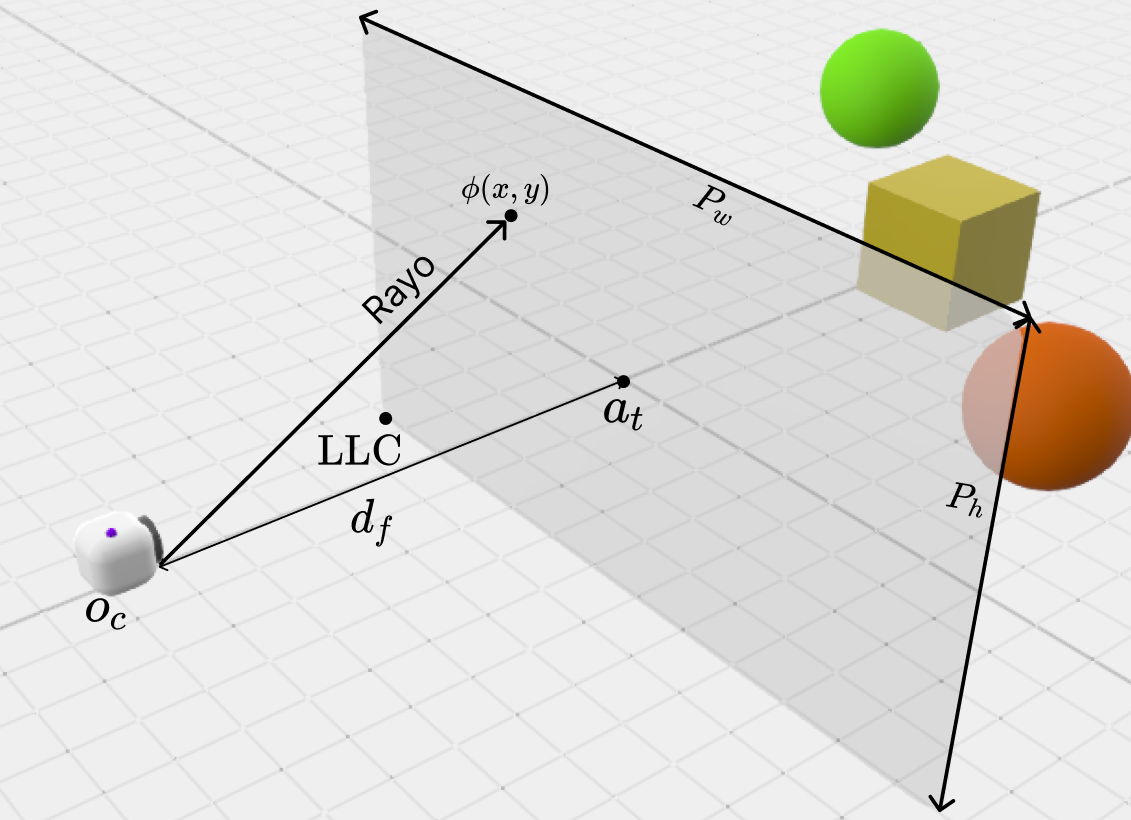
\includegraphics[width=9cm]{img/C8/elementos-PP.png}
    \caption{Elementos que participan en RT}
    \label{fig:elementos}
\end{figure}

Una vez conocemos las coordenadas de mundo de la esquina superior izquierda, la cual identificamos con el píxel inferior izquierdo del canvas, debemos recuperar la transformación \ref{eq:transformacion-lineal-3}, pero en este caso nos debemos llevar la región $[0,n_x]\times[0,n_y]$ a $[0,P_w]\times[0,P_h]\times\{-1\}$ (recordemos que estamos situando el plano de proyección en el plano $z=-1$). La transformación por tanto en este caso es

\begin{equation}
    \label{eq:transformacion-lineal-4}
    \begin{split}
        \phi : [0,n_x]\times [0,n_y] & \longrightarrow [0,P_w]\times[0,P_h]\times \{-1\} \\
        (x,y) & \longmapsto \left(\frac{P_w\cdot x}{n_x},\frac{P_h\cdot y}{n_y},-1\right)
    \end{split}
\end{equation}
donde $(x,y)$ son las coordenadas de dispositivo en términos de píxeles a las que puede acceder el fragment shader a traves de \verb|gl_FragCoor|, a las cuales recordamos que se les suele añadir $\frac{1}{2}$ en cada componente para así hacer la identificación con el punto que se encuentra en el centro del píxel, y no la esquina inferior izquierda. Así identificamos el alto y ancho del canvas con el alto y ancho del plano de proyección, de manera que a partir de estos valores y conociendo qué punto se sitúa en la esquina inferior izquierda podemos definitivamente calcular con qué punto del plano de proyección ($P$) identificamos el píxel:
\begin{equation}
    \label{eq:transformacion-lineal-5}
    \begin{split}
        \phi : [0,n_x]\times [0,n_y] & \longrightarrow P \\
        (x,y) & \longmapsto LLC + \left(\frac{P_w}{n_x}x,\frac{P_h}{n_y}y,-1\right)
    \end{split}
\end{equation}
Y por tanto, la dirección del rayo sería
$$
\vec v = \phi(x,y) - o_c
$$
y el origen sería obviamente el punto $o_c$.

Como mencionamos anteriormente, la transformación $\phi$ es la que corresponde a la inversa de la matriz $M$ de vista y proyección, pues transforma las coordenadas de dispositivo en coordenadas de mundo del plano de proyección. Suponiendo que identificamos las coordenadas de dispositivo $(x,y)$ con el vector $(x,y,0,1)^t$ y un punto $p=(p_1,p_2,p_3)\in\R^3$ con el vector $(p_1,p_2,p_3,1)^t$, la transformación (\ref{eq:transformacion-lineal-5}) puede expresarse matricialmente como:

\begin{equation}
    \label{eq:transformacion-lineal-matrix-3D-base}
    \phi(x,y) = \left(\begin{array}{ccc|c}
        \frac{P_w}{n_x} & 0 & 0 & 0 \\
        0 & \frac{P_h}{n_y} & 0 & 0 \\
        0 & 0 & 0 & -1 \\ \hline
        0 & 0 & 0 & 1
    \end{array}\right)\left(
        \begin{array}{c}
            x \\ y \\ 0 \\ \hline 1
        \end{array}\right)
\end{equation}

El código GLSL que hemos utilizado hasta este punto, en el que hemos calculado $\mathrm{LLC}$ e implementado la transformación (\ref{eq:transformacion-lineal-5}), sería el siguiente:

\begin{lstlisting}

Ray get_ray(vec3 lookfrom, vec3 lookat, 
    float viewport_width, float viewport_height, 
    float u, float v) {
    
    Ray R;
    R.orig = lookfrom;
    float df = length(lookat - lookfrom); // Distancia focal
    vec3 lower_left_corner = lookfrom
        - viewport_width/float(2.0)*vec3(1.0, 0.0, 0.0)
        - viewport_height/float(2.0)*vec3(0.0, 1.0, 0.0) 
        - df*vec3(0.0, 0.0, 1.0);
    R.dir = lower_left_corner 
        + u*vec3(viewport_width, 0.0, 0.0)
        + v*vec3(0.0, viewport_height, 0.0) 
        - lookfrom;
    return R;
}

// ... 

// Dimensiones del canvas
float aspect_ratio = 16.0/9.0;
float nx = 1280.0;
float ny = nx / aspect_ratio;

// Coordenadas de dispositivo normalizadas [0,1]
vec2 uv = (gl_FragCoord.xy + vec2(0.5)) / vec2(nx, ny);
float u = uv.x;
float v = uv.y;

// Dimensiones del plano de proyeccion
float viewport_height = float(2.0);
float viewport_width = viewport_height * aspect_ratio;

// lookfrom y lookat
vec3 lookfrom = vec3(0.0, 0.0, 0.0);
vec3 lookat = vec3(0.0, 0.0, -1.0);

// Ray
Ray R = get_ray(lookfrom, lookat, 
    viewport_width, viewport_height, 
    u, v);
\end{lstlisting}

Y de esta forma el fragment shader obtiene un rayo por cada píxel que tiene como origen la posición del observador y que interseca con el plano de proyección en el punto correspondiente al píxel.

\section{El background}

Una vez tenemos creado el rayo asignado a un píxel debemos asignar un color. La función que dado un rayo $R$ devuelve el color del cual colorearemos el píxel la llamaremos \verb|ray_color|. Esta función se verá sometida a muchos cambios, sobre todo en sus argumentos dependiendo de los elementos que compongan la escena, pero de momento asumimos una escena vacía. Que la escena esté vacía supone que ningún rayo interseca ninguna superficie, pero independientemente de ello hay que asignar un color al píxel. Esta asignación de color a un rayo que no interseca ninguna superficie determina el fondo (\textit{background}) de la escena, y esta decisión que tomaremos ahora sobre cómo colorear el fondo nos acompañará durante el resto del desarrollo. 

En concreto, hemos decidido simular algo parecido al cielo mediante un degradado vertical de un azul \texttt{rgb(127, 178, 255)} a blanco \texttt{rgb(255, 255, 255)}, definiendo el color a partir de la componente $y$ del vector director normalizado. Mostramos el código correspondiente también para clarificar esta descripción.

\begin{lstlisting}
vec4 ray_color(Ray R) {
    // R no interseca ninguna superficie
    vec3 unit_direction = normalize(R.dir);
    float t = 0.5*(unit_direction.y + 1.0);
    return vec4((1.0-t)*vec3(1.0,1.0,1.0) + t*vec3(0.5,0.7,1.0), 1.0);
}
\end{lstlisting}

De esta forma, si el rayo apunta hacia arriba el color del píxel será más azul y si apunta hacia abajo más blanco. En la imagen \ref{fig:background} podemos ver el gradiente utilizado.

\begin{figure} [ht]
    \centering
    
\includegraphics[scale = 0.35]{img/C8/background-gradient.png}
    \caption{Gradiente utilizado para el fondo de la escena}
    \label{fig:background}
\end{figure}

Y en la imagen \ref{fig:first-render} podemos ver el resultado de efectuar la llamada a \verb|ray_color| una vez creado el rayo. Esta es la primera escena 3D generada utilizando RT en WebGL. 
\begin{lstlisting}
gl_FragColor = ray_color(R);
\end{lstlisting}

\begin{figure} [ht]
    \centering
    
\includegraphics[scale = 0.35]{img/C8/first-render.png}
    \caption{Primera escena vacía visualizada}
    \label{fig:first-render}
\end{figure}

Nótese que en la imagen no aparecen todos los colores del gradiente de la imagen \ref{fig:background}, y esto se debe a que los rayos que se trazan en esta situación inicial no cubren todas las alturas posibles. Por ejemplo, no se traza un rayo totalmente vertical hacia arriba ni hacia abajo, solo se trazan las alturas necesarias para cubrir el plano de proyección. Esto nos da una manera de orientarnos en la altura una vez parametricemos la posición y orientación de la cámara (sección \ref{section:camara}), de tal manera que si vemos el fondo muy azul podemos asumir que se está mirando `al cielo' y si el color es blanco se estará mirando `al vacío'. 



\section{Visualizando una escena sencilla}
\label{section:escena}

Hasta este momento hemos diseñado la estructura del ray tracer como un observador situado en la posición $(0, 0,0)$ y proyectando una escena vacía en un plano de $2$ unidades de alto y guardando un ratio de 16:9. Sin embargo, aún queda lo más importante, que es añadir cuerpos a la escena con los que los rayos puedan intersecar. El objetivo de esta sección es describir la metodología y el código GLSL necesario para dibujar una escena con una o varias esferas y un plano con textura de tablero de ajedrez. 

Para ello, y debido a la simplicidad que requiere el cálculo de intersecciones rayo-esfera y rayo-plano, calcularemos analíticamente las intersecciones, explicando detalladamente cómo hallarlas en las secciones \ref{subsection:esfera} y \ref{subsection:plano} respectivamente. En el capítulo \ref{chap:fractales-3D} sustituimos este cálculo analítico por un cálculo iterativo utilizando el algoritmo sphere-tracing, pero a modo introductorio es más sencillo de momento calcular directamente las intersecciones.

Tras esta visualización sencilla, en la sección \ref{section:Phong} emplearemos además un modelo de iluminación local sencillo pero muy utilizado: el modelo de Phong, el cual se describe con detalle a nivel teórico y a nivel de código. Con esto completaríamos los tres ítems esenciales que mencionamos al inicio de la sección \ref{section:elementos-RT}: rayos primarios, intersecciones y MIL.

\subsection{Visualizando una esfera}
\label{subsection:esfera}

Primero introduciremos código para visualizar una esfera. Por simple geometría euclídea sabemos que, fijado un centro $c=(c_x,c_y,c_z)\in\R^3$ y un radio $r\in\R^+$, una esfera $S$ se define como aquellos puntos de $\R^3$ tales que su distancia a $c$ es $r$, es decir:
$$
S = \{p\in\R^3:\|p-c\|=r\} = \{p\in\R^3:(p-c)\cdot (p-c)=r^2\}. 
$$
donde en esta definición el operador $\cdot$ denota el producto escalar de $\R^3$. Si recordamos que los puntos que componen un rayo $R$ se pueden expresar como $R(t)= p_0 + \vec vt$ (donde $p_0$ es el origen del rayo y el vector $\vec v$ su dirección) con valores de $t$ reales no negativos, podemos calcular la intersección rayo-esfera sin más que resolver la ecuación
$$
(R(t)-c)\cdot(R(t)-c)=r^2
$$
de tal manera que, si resolvemos la ecuación en $t$ podremos saber en qué valor de $t$ golpea el rayo la esfera, si es que efectivamente lo interseca.
\begin{equation}
    \label{eq:rayo-recta}
    \begin{split}
        (R(t)-c)\cdot(R(t)-c)&=r^2 \\
        (p_0 + \vec vt - c)\cdot(p_0 + \vec vt - c) &= r^2 \\
        (\vec vt + (p_0 -c))\cdot (\vec vt + (p_0 -c))&= r^2 \\
        (\vec v\cdot \vec v)t^2 + 2(\vec v\cdot(p_0-c))t + (p_0 -c)\cdot (p_0 -c) - r^2 &= 0 
    \end{split}
\end{equation}

Y esto es una ecuación de segundo grado en $t$. Esto nos dice que el rayo puede intersecar dos veces con la esfera (secante), una única vez si el discriminante se anula (tangente) o ninguna si el discriminante es negativo (el rayo no interseca con la esfera). En caso de que exista intersección debemos quedarnos con el valor de $t$ más pequeño, que es el más cercano al punto de vista. También debemos quedarnos únicamente con valores de $t$ positivos, pues si es negativo significa que la esfera está detrás del observador, en cuyo caso no es visible.

A nivel de código podemos codificar una esfera como un \verb|struct| cuyos elementos sean su centro y su radio

\begin{lstlisting}
struct Sphere{
    vec3 center;    // Centro de la esfera
    float radius;   // Radio de la esfera
};
\end{lstlisting}

Además, para el futuro necesitaremos una estructura que almacene información sobre un impacto rayo-superficie. Información como el punto en el que se produce, en qué $t$, la normal a la superficie en ese punto, etc. En estas fases tan tempranas igual no es tan necesario pero pronto encontraremos su utilidad.

\begin{lstlisting}
struct Hit_record {
    vec3 p;         // Punto donde se produce el impacto
    vec3 normal;    // Normal a la superficie en el punto p
    float t;        // Valor de t para el que el rayo impacta
    bool hit;       // True sii se golpea alguna superficie
};
\end{lstlisting}

Claro que los tres primeros campos solo tendrán sentido si el campo \verb|hit| es verdadero, si es falso no tiene sentido calcular ni consultar los demás. A continuación presentamos el código GLSL para visualizar una esfera utilizando estas estructuras.

\begin{lstlisting}
// Calcula la interseccion entre un rayo y una esfera
// y almacena la informacion del impacto en una
// estructura Hit_record
Hit_record hit_sphere(Sphere S, Ray R, 
    float t_min, float t_max) {

    Hit_record result;
    vec3 oc = R.orig - S.center;
    float a = dot(R.dir, R.dir);
    float b = 2.0 * dot(oc, R.dir);
    float c = dot(oc, oc) - S.radius*S.radius;
    float discriminant = b*b - 4.0*a*c;
    if (discriminant < 0.0){
        result.hit = false;
        return result;
    }
    float sqrtd = sqrt(discriminant);
    float root = (-b - sqrt(discriminant))/(2.0*a); // Primera raiz
    if (root < t_min || t_max < root){ 
        // La primera raiz esta fuera del rango que nos interesa
        root = (-b + sqrt(discriminant))/(2.0*a); // La otra raiz
        if(root < t_min || t_max < root){ 
            // Las dos raices estan fuera del rango,
            // consideramos que no existe impacto
            result.hit = false;
            return result;
        }
    } 
    result.hit = true;
    result.t = root;
    result.p = ray_at(R, result.t);
    result.normal = normalize((result.p - S.center) / S.radius);
    return result;
}
\end{lstlisting}

Fijémonos en que hemos introducido unas variables \verb|t_min| y \verb|t_max| de forma que sólo nos interesamos por los puntos del rayo $R(t)=p_0+\vec vt$ para valores de $t$ situados entre un valor mínimo y un máximo. Esto sirve para fijar una distancia mínima y máxima en la que buscar intersecciones, evitando así valores de $t$ negativos o demasiado grandes. El código implementa la ecuación (\ref{eq:rayo-recta}) de forma que en caso de no haber impacto asigna \verb|false| al campo \verb|hit| de la estructura \verb|Hit_record| y \verb|true| en caso contrario. Además, solo calcula el punto de intersección más cercano.

A partir de la estructura \verb|Hit_record| y la información que contiene podemos asignar el color que deseemos. Lo ideal es evaluar un modelo de iluminación, como haremos en la sección \ref{section:Phong}, pero de momento aprovecharemos la normal en cada punto para mapear una componente de $\R^3$ normalizada en una terna RGB. Esto es una forma de simular un material conocido popularmente como `\textit{normal material}'\footnote{Consultar por ejemplo la implementación en Three.js para más información \url{https://threejs.org/docs/\#api/en/materials/MeshNormalMaterial}}, llamado así por utilizar la normal en un punto para calcular un color.

Realizamos por tanto la primera modificación del código de \verb|ray_color|, que ahora acepta como argumento una esfera.

\begin{lstlisting}
// Fijamos una distancia maxima
#define MAX_DIST 100.0

// ... 

vec4 ray_color(Ray R, Sphere S) {

    // R interseca la esfera?
    Hit_record hr = hit_sphere(S, R, 0.0, MAX_DIST);
    if(hr.hit){
        // Nos llevamos las componentes a [0,1]
        vec3 color = (hr.normal + vec3(1.0))/float(2.0);
        return vec4(color, 1.0);
    }

    // R no interseca ninguna superficie
    vec3 unit_direction = normalize(R.dir);
    float t = 0.5*(unit_direction.y + 1.0);
    return vec4((1.0-t)*vec3(1.0,1.0,1.0) + t*vec3(0.5,0.7,1.0), 1.0);
}

// ... 
// R es el rayo (Ray)

Sphere S; 
S.center = vec3(0.0, 0.0, -1.0); S.radius = 0.5;
gl_FragColor = ray_color(R, S);
\end{lstlisting}

El resultado que obtenemos es el que podemos observar en la imagen \ref{fig:una-esfera}. Obsérvese la variedad de colores que ofrece la esfera, concordante con la variedad de normales que posee.

\begin{figure} [ht]
    \centering
    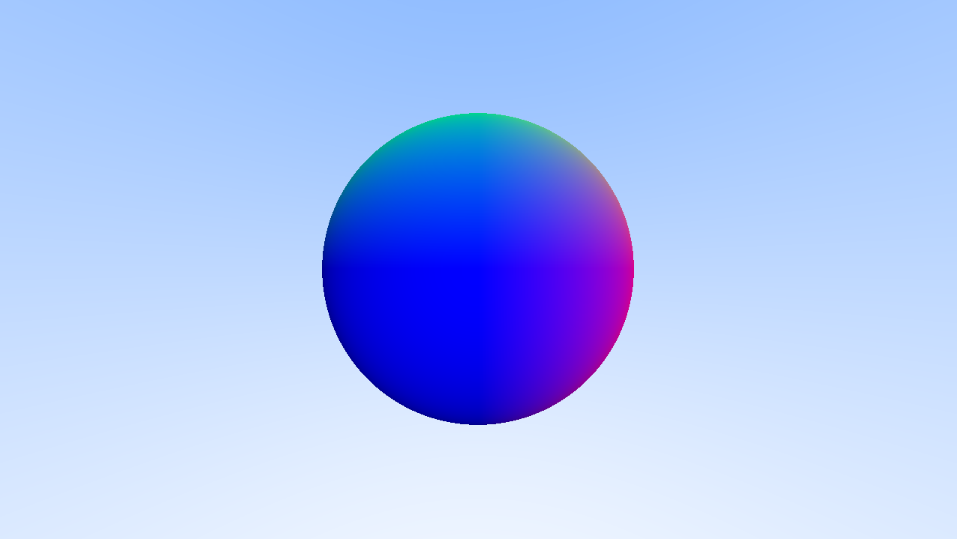
\includegraphics[scale = 0.3]{img/C8/esfera_renderizada.png}
    \caption{Escena con una esfera}
    \label{fig:una-esfera}
\end{figure}

\subsection{Visualizando varias esferas}

Veamos ahora cómo poder visualizar varias esferas, aunque el procedimiento una vez se ha conseguido visualizar una es bastante natural. Podemos declarar en lugar de una un array de esferas, cada una con sus parámetros y crear una función que itere llamando a la función \verb|hit_sphere| con cada esfera. Sin embargo, un rayo puede intersecar varias esferas, pero consideramos que únicamente hemos golpeado la más cercana a efectos prácticos. Este problema se extiende en general a escenas con varios objetos, no sólo esferas, pero la solución es la misma, evaluar únicamente la más cercana de las intersecciones. Aquí es también donde ponemos en valor el parámetro \verb|t_max| de la función \verb|hit_sphere|, pues una vez hemos encontrado una intersección con una de las esferas no debemos considerar impactos más lejanos.

Por tanto, buscamos implementar una función que dado un array de esferas devuelva en una estructura \verb|Hit_record| la información sobre la intersección rayo-esfera con el valor de $t$ más pequeño. El método consiste en llamar a \verb|hit_sphere| almacenando la información de la intersección pero sólo mantenemos la información de la más próxima, buscando en cada iteración únicamente intersecciones más cercanas que las anteriores (en caso de haberlas).
\begin{lstlisting}
// Tamano de los arrays
#define ARRAY_TAM 100

// ... 

Hit_record hit_spheres_list(Sphere spheres[ARRAY_TAM], 
    int size, Ray R, float t_min, float t_max) {

    Hit_record result, tmp;
    result.hit = false;
    float closest_t = t_max;
    for(int i = 0; i < ARRAY_TAM; i++){
        if(i == size) break;
        // Buscamos tan lejos como la ultima interseccion
        tmp = hit_sphere(spheres[i], R, t_min, closest_t);
        if(tmp.hit){    // Hay una interseccion mas cercana
            closest_t = tmp.t;
            result = tmp;
        }
    }
    return result;
}
\end{lstlisting} 

Y en la función \verb|main| inicializamos algunas esferas, editamos \verb|ray_color| para que acepte como argumento un array de esferas y desde ahí hacemos llamada a \verb|hit_spheres_list|.

\begin{lstlisting}
vec4 ray_color(Ray R, Sphere world[ARRAY_TAM], int size) {

    // R interseca alguna superficie?
    Hit_record hr = hit_spheres_list(world, size, R, 0.0, MAX_DIST);
    if(hr.hit)
        return vec4((hr.normal+vec3(1.0))/2.0, 1.0);

    // R no interseca ninguna superficie
    // Codigo del background ... 
}

// ... 
// R es el rayo (Ray)

// Esferas
int num_spheres = 4;
Sphere world[ARRAY_TAM];
Sphere S1, S2, S3, S4;
S1.center = vec3(0.0, 0.0, -1.0);   S1.radius = 0.5; 
S2.center = vec3(-5, 0.5, -3.0);    S2.radius = 4.0;
S3.center = vec3(2.0, -3, -4.0);    S3.radius = 1.5;
S4.center = vec3(20.0, 10, -20.0);  S4.radius = 3.0;
world[0] = S1; world[1] = S2; world[2] = S3; world[3] = S4;

gl_FragColor = ray_color(R, world, num_spheres);

\end{lstlisting}

Y así obtenemos la imagen \ref{fig:varias-esferas}, en la que podemos ver varias esferas de distintos tamaños y con distintas posiciones.

\begin{figure} [ht]
    \centering
    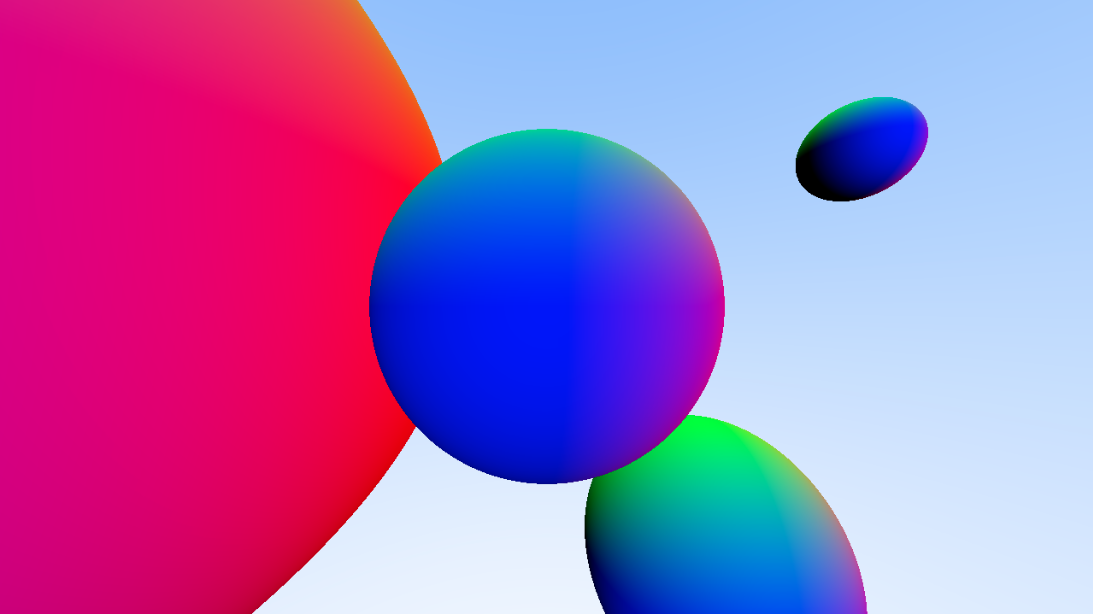
\includegraphics[scale = 0.25]{img/C8/varias-esferas.png}
    \caption{Escena con varias esferas}
    \label{fig:varias-esferas}
\end{figure}

\subsection{Visualizando un plano con textura de ajedrez}
\label{subsection:plano}

Para orientarnos en la escena cuando podamos modificar la posición de la cámara dinámicamente y hacernos también a la idea del movimiento que estamos haciendo y a qué velocidad es útil utilizar un plano con textura similar a la de un tablero de ajedrez a modo de suelo. Necesitamos por tanto ahora implementar la intersección rayo-plano y una vez encontrada la intersección discernir entre colorear el punto negro o blanco.

En geometría euclídea una forma de caracterizar los puntos de un plano $P$ es mediante una ecuación lineal
$$
P = \{(x,y,z)\in\R^3:Ax+By+Cz=D\}
$$
donde el vector $\vec N=(A,B,C)\in\R^3$ es un vector normal al plano ($-(A,B,C)$ también lo sería) y $D\in\R$ es una constante que define la posición del plano. Podemos entonces ver un plano de la siguiente forma equivalente
$$
P = \{p=(x,y,z)\in\R^3:\vec N\cdot p = D\}
$$
donde de nuevo el punto $\cdot$ denota el producto escalar. Si ahora queremos calcular la intersección del plano $P$ con un rayo $R(t)=p_0+\vec vt$ tenemos que resolver una ecuación que además es lineal:
\begin{equation}
    \label{eq:plano-recta}
    \begin{split}
        R(t)\cdot \vec N &= D \\
        (p_0+\vec vt)\cdot \vec N & = D\\
        t &=\dfrac{D-p_0\cdot \vec N}{\vec v\cdot \vec N}
    \end{split}
\end{equation}
Lo cual nos dice en qué $t$ se produce la intersección. Obsérvese que en el caso de que la dirección del rayo $\vec v$ y la normal al plano $\vec N$ sean perpendiculares (\textit{i.e.} $\vec v\cdot N=0$), lo cual se traduce en que el rayo es paralelo al plano o está incluido en el mismo, no existe intersección.

Como ya hemos dicho, podemos identificar unívocamente un plano a partir de su normal en cualquier punto y una constante $D\in\R$, por lo que mediante una estructura podemos representar en GLSL un plano.

\begin{lstlisting}
struct Plane{
    vec3 normal;    // Vector normal al plano
    float D;        // Termino independiente
};
\end{lstlisting}

Y a partir de la ecuación (\ref{eq:plano-recta}) podemos implementar la función \verb|hit_plane|, que hace lo correspondiente a \verb|hit_sphere| pero acepta como argumento un plano y devuelve la intersección con el mismo.

\begin{lstlisting}
Hit_record hit_plane(Plane P, Ray R, float t_min, float t_max){
    Hit_record result;
    float oc = dot(P.normal, R.dir);
    if(oc == 0.0){  // No hay interseccion
        result.hit = false;
        return result;
    }
    float t = (P.D - dot(P.normal, R.orig))/oc;
    if (t < t_min || t > t_max)
        result.hit = false;
    else{
        result.hit = true;
        result.t = t;
        result.p = ray_at(R, result.t);
        result.normal = normalize(P.normal);
    }
    return result;
}
\end{lstlisting}

Y ahora desde \verb|ray_color| debemos considerar la posibilidad de intersecar con el plano o con las esferas, pero solo debemos darle color a la intersección más próxima. Por eso debemos mantener una variable \verb|t_closest| que represente el valor de $t$ más pequeño en el que hemos detectado una intersección. Puede ocurrir que el rayo impacte primero con una esfera y después con el plano o al revés, primero el plano y después una esfera; en estos casos se daría color atendiendo la intersección con la esfera y con el plano respectivamente. 

Como es natural, utilizaremos como suelo un plano horizontal, como puede ser el plano $P=\{(x,y,z)\in\R^3:y=-2\}$, en cuyo caso $\vec N=(0,1,0)$, $D=-2$. Véamos entonces cómo aplicarle una textura a este plano. Normalmente las texturas se suelen almacenar en imágenes, pero por sencillez en este caso la generaremos proceduralmente desde el fragment shader. Es decir, se evalúa el color de la textura en función del punto en la superficie del objeto, de forma que a cada punto del plano le asignamos un color (blanco o negro). 

Por tanto, se trata de un algoritmo que a partir de una coordenada 2D de un punto en el suelo $(u,v)$ se calcula una terna RGB de color, que es el que se asigna finalmente al píxel. Los puntos de $P$ son de la forma $(x,-2,z)$, con $ x,z\in\R$, y utilizaremos como coordenadas $(u,v)$ a los pares $(x,z)$ extraídos de las coordenadas de mundo $(x,y,z)$ de los puntos que forman el plano. Muchas veces, sobre todo en superficies que no son planas o que son irregulares, el mapeo $(x,y,z)\longmapsto(u,v)$ es mucho más complejo, pero en este caso es bastante sencillo.

Lo primero es quedarnos con la parte entera de ambos valores, de forma que dividimos el plano en cuadrados. Si la suma de las partes enteras es un número par, colorearemos el píxel de blanco, y si es impar de negro. En la imagen \ref{fig:ajedrez} podemos ver cómo identificando cada punto con las partes enteras de cada componente y coloreando de negro las partes enteras cuya suma sea impar se obtiene una textura de ajedrez.

\begin{figure} [ht]
    \centering
    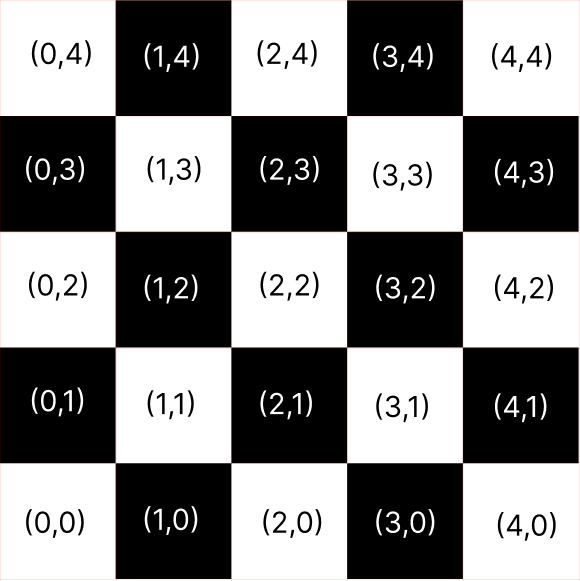
\includegraphics[scale = 0.25]{img/C8/ajedrez.png}
    \caption{Textura de ajedrez a partir de las partes enteras}
    \label{fig:ajedrez}
\end{figure}

Debemos, por tanto, en \verb|ray_color| añadir esta funcionalidad.

\begin{lstlisting}
vec4 ray_color(Ray r, Sphere world[ARRAY_TAM], 
    int size, Plane P) {
    
    float t_closest = MAX_DIST;   
    // r interseca alguna esfera?
    vec4 tmp_color;
    Hit_record hr = hit_spheres_list(world, size, r, 0.0, t_closest);
    if(hr.hit){
        t_closest = hr.t;
        tmp_color = vec4((hr.normal + vec3(1.0))/2.0, 1.0);
    }

    // r interseca el plano?
    // Solo intersecciones mas cercanas
    hr = hit_plane(P, r, 0.0, t_closest);
    if(hr.hit){
        t_closest = hr.t;
        vec3 p = hr.p;
        int x_int = int(floor(p.x)), // Parte entera de x
            z_int = int(floor(p.z)), // Parte entera de z
            sum = x_int + z_int;     // Suma de partes enteras
        // Modulo 2
        int modulus = sum - (2*int(sum/2));
        if(modulus == 0)    // Suma par
            tmp_color = vec4(1.0, 1.0, 1.0, 1.0);
        else                // Suma impar
            tmp_color = vec4(0.0,0.0,0.0, 1.0);
    }
    // Si r interseca alguna superficie
    if(t_closest < MAX_DIST) return tmp_color;
    // r no interseca ninguna superficie
    // Codigo del background ... 
}
\end{lstlisting}

Y tras declarar el plano $y=-2$, las esferas y realizar la llamada a \verb|ray_color|, al fin podemos visualizar una escena completa compuesta de varias esferas y un plano, tal y como nos propusimos al inicio de esta sección \ref{section:escena}

\begin{lstlisting}
// ... 
// R es el rayo (Ray)
// world es el array de objetos 'Sphere'

// Plano
Plane P;
P.normal = vec3(0.0, 1.0, 0.0);
P.D = -2.0;     // y = -2.0

gl_FragColor = ray_color(r, world, num_spheres, P);
\end{lstlisting}

\begin{figure} [ht]
    \centering
    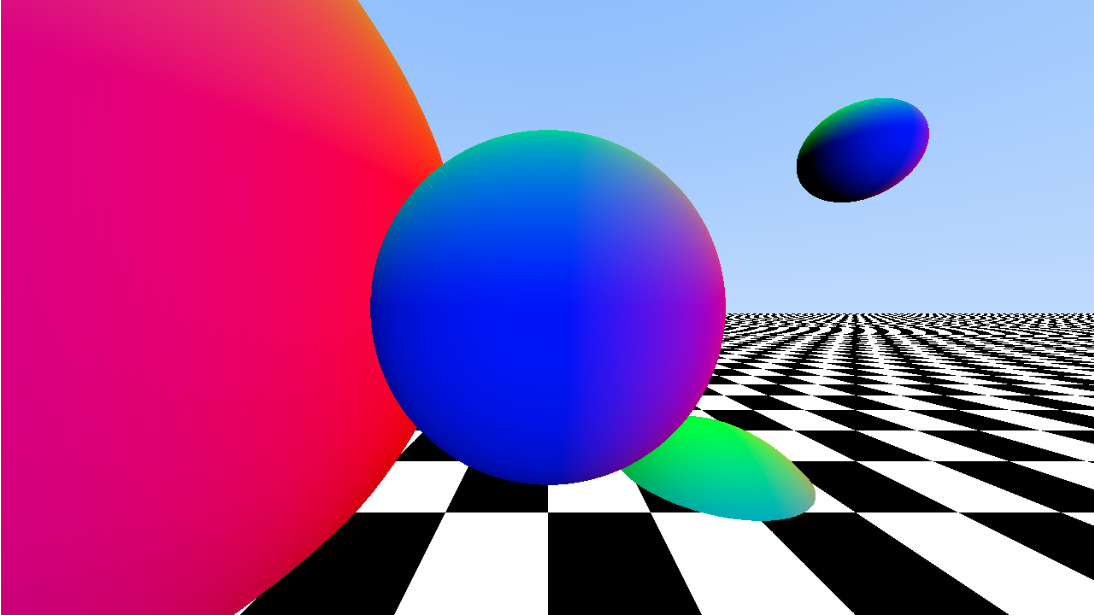
\includegraphics[scale = 0.25]{img/C8/escena-completa.png}
    \caption{Escena compuesta por esferas y un plano}
    \label{fig:escena-completa}
\end{figure}

\section{Configurando la cámara}
\label{section:camara}

Hasta ahora hemos visto cómo componer una escena sencilla y visualizarla, pero desde el principio nos hemos visto limitados por la decisión que tomamos de situar al observador en el punto $(0,0,0)$, mirar hacia el $(0,0,-1)$ y proyectar la escena en un plano de altura $2$ y ratio $16:9$. Evidentemente una aplicación gráfica en la que tanto el observador como la escena se mantienen fijos carece de interés alguno. Debemos añadir la posibilidad de modificar la posición del observador y la dirección en la que se mira, para así poder disfrutar de distintos puntos de vista en una misma escena.

Lo primero es fijar una serie de conceptos. Recordamos que denominábamos \textit{lookfrom} al punto desde el cual se observa ($o_c$), es decir, el punto de vista; y \textit{lookat} al punto sobre el cual se fija la mirada ($a_t$). Nótese que realmente el punto $a_t$ puede ser cualquiera situado en la semirrecta que une al observador y el centro del plano de proyección, no tiene por qué estar incluido como tal en el propio plano de proyección; pensemos en alguna vez que hemos pensado que alguien nos saludaba y realmente saludaba a alguien que está detrás nuestra.

Se denomina \textit{field of view (FOV)} al ángulo total observable, que corresponde al ángulo $\theta$ en la imagen \ref{fig:fov}. Como nuestro plano de proyección no es cuadrado, este ángulo es distinto en vertical y en horizontal, pero del ratio $16:9$ ($r=16/9$) se deduce el uno del otro. En nuestro caso fijaremos $\theta=90^\circ=\pi/2 \rad$, sea $h=\tan\left(\frac \theta 2\right)=1$ el ratio constante que van a mantener la semialtura del plano de proyección y la distancia focal, tal y como se puede observar en la imagen \ref{fig:fov}. Nosotros mantendremos entonces fijas la altura del plano de proyección $P_h=2=2h$ y la distancia focal $d_f=1=h$.

\begin{figure} [ht]
    \centering
    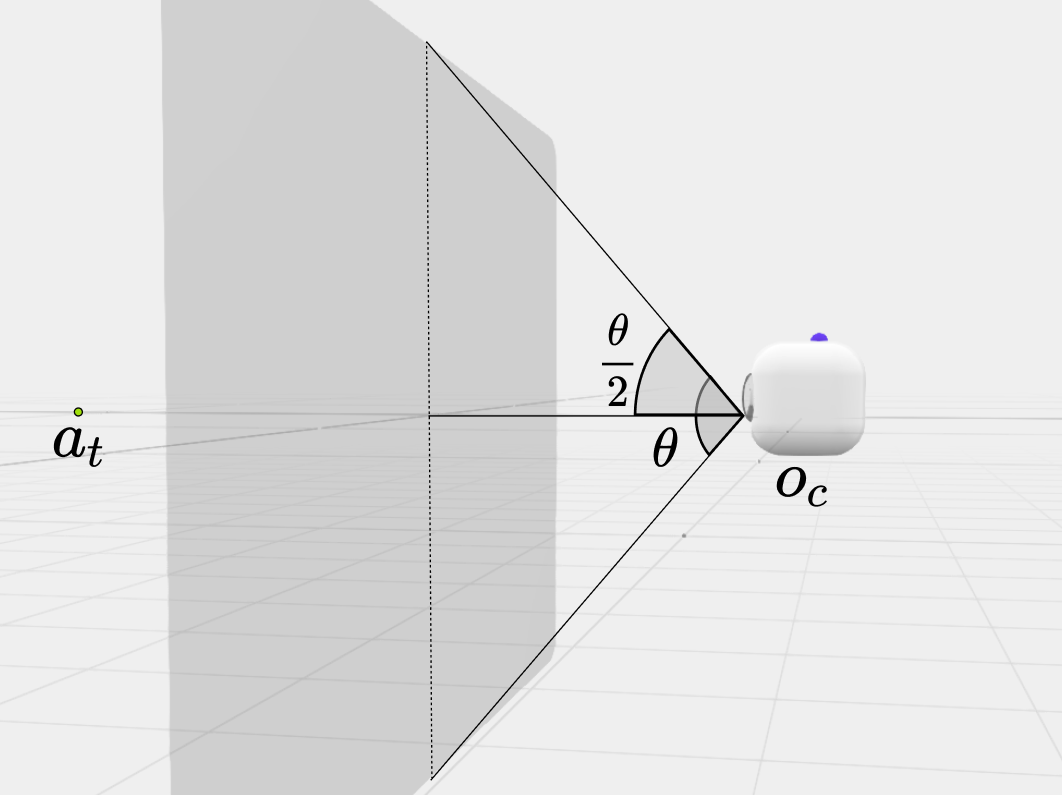
\includegraphics[scale = 0.25]{img/C8/fov.png}
    \caption{Field Of View}
    \label{fig:fov}
\end{figure}

Por otro lado, aunque definamos un punto desde el que mirar y un punto al que mirar, no está todo dicho sobre la orientación de la cámara. Piense que mientras usted lee este documento puede girar la cabeza hacia un lado y seguir mirando desde y hacia la misma posición. Por tanto necesitamos alguna forma de expresarle a la cámara que se mantenga vertical. Esto se hace mediante un vector que se denomina \textit{view up} ($\overrightarrow{\mathrm{vup}}$), el cual define ese `arriba' para la cámara. Normalmente, por convención se hace la elección $\overrightarrow{\mathrm{vup}}=(0,1,0)$. Mediante el vector $\vec{v}_d=o_c-a_t$ (\textit{view direction}) y el vector $\overrightarrow{\mathrm{vup}}$ podemos crear un sistema de referencia ortonormal del plano ortogonal a $\vec{v}_d$ que pasa por el punto $o_c$ y que define la orientación de la cámara. No confundamos este plano con el plano de proyección, pues aunque vectorialmente son iguales, y son por tanto paralelos desde el punto de vista afín, son planos distintos. Precisamente de este hecho nos aprovecharemos más tarde. Presentamos entones los siguientes vectores
\begin{eqnarray*}
    \vec w = \dfrac{o_c-a_t}{\|o_c-a_t\|}, \\
    \vec u = \dfrac{\overrightarrow{\mathrm{vup}}\times \vec w}{\|\overrightarrow{\mathrm{vup}} \times \vec w\|}, \\
    \vec v = \vec w\times \vec u,
\end{eqnarray*}
de forma que los vectores $\vec u,\vec v$ son, por su propia definición ortogonales a $\vec{v}_d$ y ortogonales entre sí. Además están normalizados, constituyendo así una base ortonormal del plano vectorial que define el plano de proyección, por lo que hacen las veces de los vectores $(1,0,0)$ y $(0,1,0)$ en el código de \verb|get_ray| en la sección \ref{section:rayo}, mientras que $\vec w$ por su parte toma el relevo del vector $(0,0,1)$. Fíjese para mejor comprensión en la imagen \ref{fig:vectores}. El conjunto $\{o_c; \vec u, \vec v,\vec w\}$ es por tanto un sistema de referencia del plano afín paralelo al plano de proyección que pasa por el punto $o_c$, al cual se le suele denominar \textit{marco de coordenadas de vista}.

\begin{figure} [ht]
    \centering
    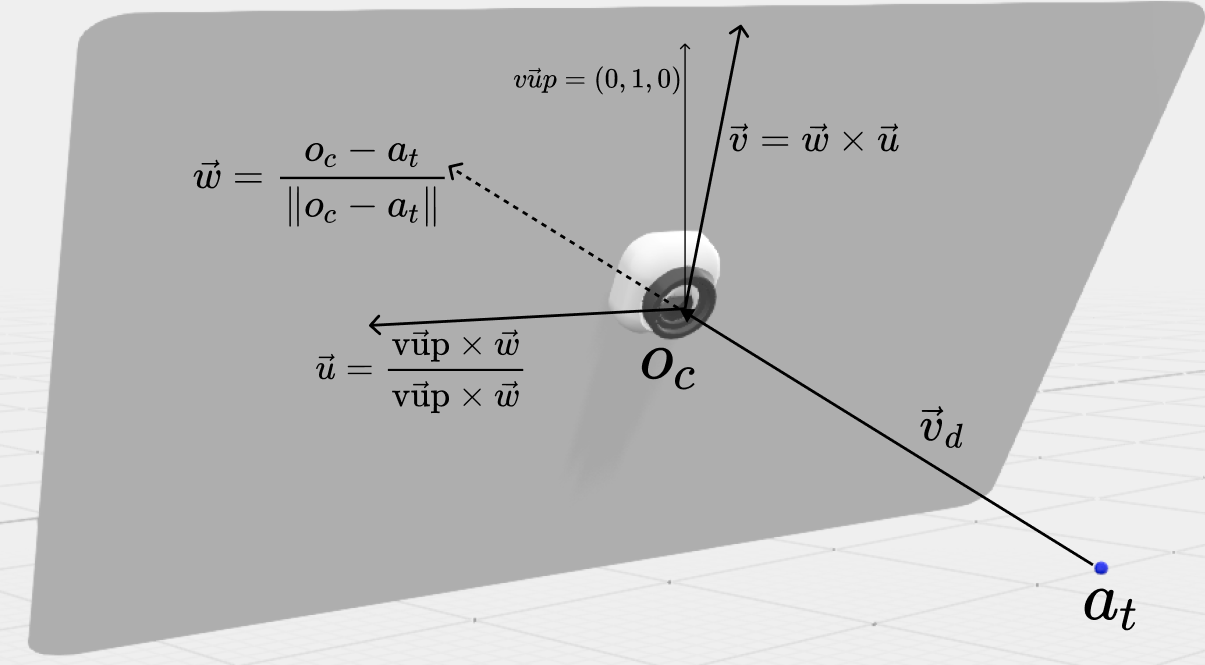
\includegraphics[scale = 0.25]{img/C8/plano.png}
    \caption{Vectores que forman una base del plano de proyección}
    \label{fig:vectores}
\end{figure}

Ahora recordamos que para crear el rayo en la seccion \ref{section:rayo} calculamos la esquina inferior izquierda, transformamos las coordenadas de dispositivo en coordenadas de mundo del plano de proyección en $[0,P_w]\times[0,P_h]\times\{-1\}$ y con ello calculamos el punto destino. En el caso generalizado la metodología es la misma, pero necesitamos aclarar, a partir de los datos de entrada como son el punto $o_c$, el punto $a_t$, el vector $\overrightarrow{\mathrm{vup}}$ (usualmente (0,1,0)), el ángulo $\widehat{\mathrm{fov}}$ y el el ratio $r$ ancho/alto (16/9 en nuestro caso), cuáles son las dimensiones del plano de proyección y la esquina inferior izquierda. Para ello introducimos una estructura que representará una cámara, que almacena los siguientes campos:

\begin{lstlisting}
struct Camera{
    vec3 origin;        // Punto desde el que se observa
    vec3 horizontal;    // Vector horizontal de modulo P_w
    vec3 vertical;      // Vector vertical de modulo P_h
    vec3 lower_left_corner; // Punto situado en la esquina
};
\end{lstlisting}
donde \verb|origin| son las coordenadas de mundo del punto en el que se sitúa la cámara, \verb|horizontal| es un vector cuyo módulo es el ancho del plano de proyección y su dirección el vector $u$ recién presentado, análogamente \verb|vertical| es un vector cuyo módulo es la altura del plano de proyección y su vector director es $v$, por último \verb|lower_left_corner| son las coordenadas de mundo del punto situado en la esquina inferior izquierda del plano de proyección. Fíjese en la imagen \ref{fig:camera-fields}.

\begin{figure} [ht]
    \centering
    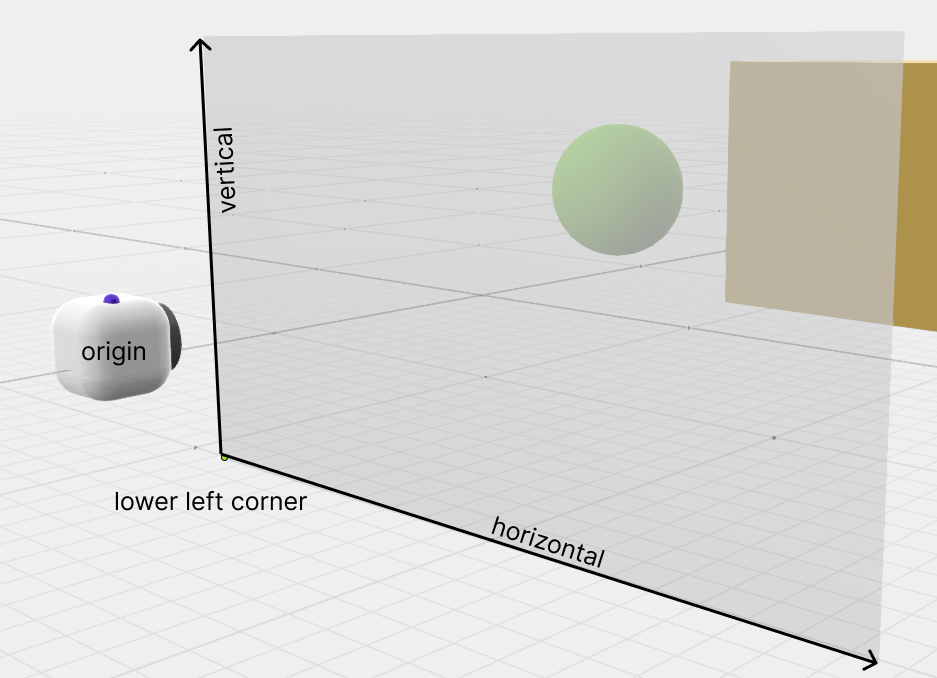
\includegraphics[scale = 0.3]{img/C8/camera-fields.png}
    \caption{Representación gráfica de los campos de `Camera'}
    \label{fig:camera-fields}
\end{figure}


Es claro que el origen es el punto \textit{lookfrom} ($o_c$), el vector horizontal es $P_w\cdot \vec u$ y el vector vertical es $P_h\cdot \vec v$. Por tanto, asumiendo una distancia focal de $1$, la esquina inferior izquierda sería
$$
\mathrm{LLC} = o_c - \frac{P_w}{2}\cdot \vec u - \frac{P_h}{2}\cdot \vec v - \vec w.
$$

En base a estos elementos, volvemos a redefinir la transformación $\phi$, de forma que ahora el plano de proyección $P$ puede tener cualquier posición y orientación. A partir de los puntos $o_c$ y $a_c$ y el vector $\overrightarrow{\mathrm{vup}}$ podríamos calcular los vectores $\vec u, \vec v, \vec w$, y como $P$ es paralelo al plano de la imagen \ref{fig:vectores}, tenemos que $\mathcal{R}=\{LLC; \vec u, \vec v, \vec w \}$ es un marco de referencia del plano de proyección, de forma que podemos obtener un punto del plano de proyección $P$ a partir de las coordenadas de dispositivo aplicando la siguiente transformación.

\begin{equation}
    \label{eq:transformacion-lineal-6}
    \begin{split}
        \phi : [0,n_x]\times [0,n_y] & \longrightarrow P \\
        (x,y) & \longmapsto LLC + \frac{P_w}{n_x}x\cdot \vec u + \frac{P_h}{n_y}y\cdot\vec v.
    \end{split}
\end{equation}

También podemos expresar esta transformación matricialmente. En este caso, la inversa de la matriz $M$ de vista y proyección se obtiene mediante el producto de la matriz de cambio de marco de referencia entre el marco usual y el marco $\mathcal{R}$ y una matriz análoga a la de la transformación (\ref{eq:transformacion-lineal-matrix-3D-base}). Realmente esto es intuitivo, pues no es más que un cambio de posición y orientación respecto al caso base.

\begin{equation}
    \label{eq:transformacion-lineal-matrix-3D-camara}
    \phi(x,y) = \left(\begin{array}{ccc|c}
        &  &  &  \\
        \vec u & \vec v & \vec w & \mathrm{LLC} \\
        &  &  &  \\ \hline
        0 & 0 & 0 & 1
    \end{array}\right)\left(\begin{array}{ccc|c}
        \frac{P_w}{n_x} & 0 & 0 & 0 \\
        0 & \frac{P_h}{n_y} & 0 & 0 \\
        0 & 0 & 0 & 0 \\ \hline
        0 & 0 & 0 & 1
    \end{array}\right)\left(
        \begin{array}{c}
            x \\ y \\ 0 \\ \hline 1
        \end{array}\right)
\end{equation}

Reflejamos estos cálculos y asignaciones en el siguiente código, que corresponde a una función que dados los parámetros de una escena, crea, inicializa y devuelve un objeto \verb|Camera|.
\begin{lstlisting}
Camera init_camera (vec3 lookfrom, vec3 lookat, 
    vec3 vup, float vfov, 
    float aspect_ratio){
    
    Camera cam;
    float focal_length = 1.0;
    float theta = degrees_to_radians(vfov); // FOV vertical
    float h = tan(theta/2.0);
    // Dimensiones del plano de proyeccion
    float viewport_height = 2.0*h*focal_length;
    float viewport_width = aspect_ratio * viewport_height;

    vec3 w = normalize(lookfrom - lookat);
    vec3 u = normalize(cross(vup,w));
    vec3 v = cross(w,u);

    cam.origin = lookfrom;
    cam.horizontal = viewport_width * u;
    cam.vertical = viewport_height * v;
    cam.lower_left_corner = cam.origin 
        - cam.horizontal/float(2.0) 
        - cam.vertical/float(2.0)
        - w;

    return cam;
}
\end{lstlisting}

Y una vez tenemos estos parámetros almacenados en un objeto \verb|Camera| la función \verb|get_ray|, a la cual ahora en lugar de todos los parámetros con la cual la programamos primitivamente en la sección \ref{section:rayo} la reprogramaremos para que acepte únicamente como argumentos la cámara y las coordenadas de dispositivo normalizadas $[0,1]$. Tomará estas coordenadas $u,v\in[0,1]$ y multiplicará por los vectores horizontal y vertical respectivamente, definiendo así el destino del rayo.

\begin{lstlisting}
Ray get_ray(Camera cam, float u, float v){
    Ray R;
    R.orig = cam.origin;
    R.dir = cam.lower_left_corner 
        + u*cam.horizontal + v*cam.vertical 
        - cam.origin;
    return R;
}
\end{lstlisting}

Vemos que ahora son los vectores \verb|cam.horizontal| y \verb|cam.vertical| los que hacen la función que en la primera implementación hacian los vectores \verb|vec3(viewport_width, 0.0, 0.0)| y \verb|vec3(0.0, viewport_height, 0.0)|.

Con todo este código, tan solo tenemos que fijar los argumentos de \verb|init_camera| y observar cómo cambia el punto de vista aunque la escena sea la misma. En principio vamos a mantener constantes el $\widehat{\mathrm{fov}}=90^\circ$, el vector $\overrightarrow{\mathrm{vup}}=(0,1,0)$ y el ratio 16:9, pero como nos gustaría poder movernos con libertad por la escena, declararemos dos variables \verb|uniform| que representen el punto $o_c$ y el punto $a_t$, a las cuales podremos asignarle variables dinámicamente desde JavaScript y dar la sensación de movimiento.

\begin{lstlisting}

uniform vec3 u_lookfrom;    // Punto lookfrom
uniform vec3 u_lookat;      // Punto lookat

// ... 
// aspect_ratio = 16/9
// nx = 1280 pixels
// ny = 720 pixels

// CAMARA
vec3 vup = vec3(0.0, 1.0, 0.0);
float vfov = 90.0; // Vertical field of view in degrees
Camera cam = init_camera(u_lookfrom, u_lookat, 
    vup, vfov, aspect_ratio);

// Coordenadas de dispositivo normalizadas [0,1]
vec2 uv = (gl_FragCoord.xy + vec2(0.5)) / vec2(nx, ny);
float u = uv.x;
float v = uv.y;

Ray r = get_ray(cam, u, v);
\end{lstlisting}

Por ejemplo, si fijamos $o_c = (1,1,1)$ y $a_t = (0,0,0)$ obtenemos la imagen \ref{fig:escena-camara} (a), y con $o_c=(5, 5, -5)$, $a_t=(1,2,-5)$ la imagen \ref{fig:escena-camara} (b). En este último caso podemos de hecho ver la escena desde el lado negativo del eje $Z$, lo que antes de parametrizar la cámara llamábamos `el interior de la pantalla'.

\begin{figure}[ht]
    \centering
    \begin{tabular}{cc}
          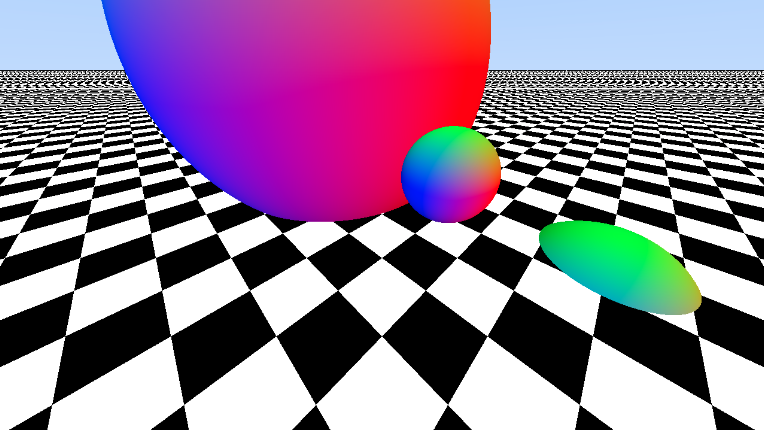
\includegraphics[scale=0.25]{img/C8/camera-1.png} &   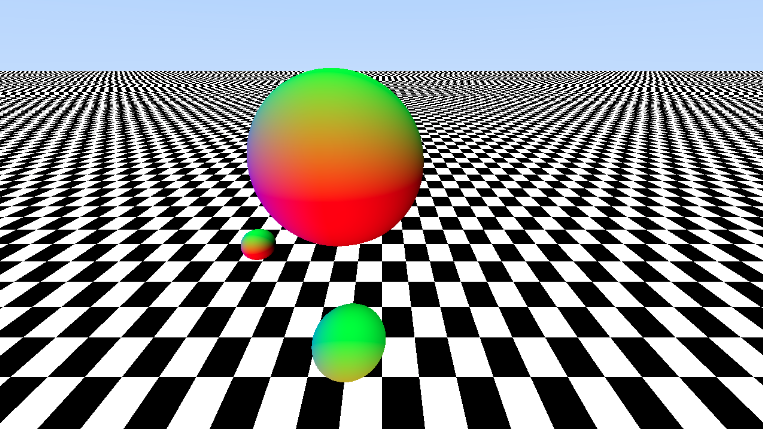
\includegraphics[scale=0.25]{img/C8/camera-2.png} \\
    (a) & (b)\\[6pt]
    \end{tabular}
    \caption{Escena \ref{fig:escena-completa} desde otros puntos de vista}
    \label{fig:escena-camara}
\end{figure}

\section{Modelo de iluminación de Phong}
\label{section:Phong}
En este punto hemos creado una escena sencilla y podemos movernos libremente por ella, pero vendría bien una dosis de realismo a la escena. Para ello, dotaremos a la escena de fuentes de luz y añadiremos a los objetos que componen la escena un material que nos permita observar su aspecto más allá del material normal que definimos en la sección \ref{subsection:esfera} a la hora de darle color a la esfera.

La iluminación real es imposible de simular porque cada punto de cada objeto irradia una cantidad de luz en todas las direcciones que es inviable de computar, por ello necesitamos de aproximaciones que simulen en mayor o menor medida dicha iluminación. Existen muchos y muy distintos modelos de iluminación, tan complejos y realistas como queramos. El conocido \textit{modelo de Phong} no es ni el más realista, ni el más complejo, pero es suficiente para nuestro cometido, pues nos permite darle colores a los materiales y apariencias mate además de posibles brillos que consiguen efectos metalizados.

Primero de todo, haremos una clasificación de los distintos modelos de iluminación que se suelen utilizar en informática gráfica en base a la luz que recibe un punto de una superficie, la cual puede deberse a:
\begin{itemize}
    \item \textbf{Iluminación directa}: Provocada por una fuente de luz que incide directamente sobre dicho punto.
    \item \textbf{Iluminación indirecta}: Luz que llega a la superficie tras haber rebotado en otras superficies.
\end{itemize}
Como consecuencia de esta clasificación, los modelos de iluminación pueden clasificarse en:
\begin{itemize}
    \item \textbf{Modelos locales}: Únicamente consideran la iluminación directa
    \item \textbf{Modelos globales}: Consideran tanto iluminación directa como indirecta.
\end{itemize}
El modelo de Phong es un modelo de iluminación local, es decir, tan solo consideraremos la posible acción directa de una fuente de luz sobre los objetos, lo cual es además computacionalmente más sencillo. Este modelo se basa en descomponer la luz que incide sobre un punto de un objeto en tres componentes RGB: ambiental, difusa y especular.

Consideraremos también únicamente el efecto de luces direccionales, las cuales se componen, tal y como su propio nombre indica, de un vector director $\vec L_p\in\R^3$ y de una tripleta RGB que es la intensidad de la luz $I_p$. El rasgo principal de este tipo de fuentes de luz es que inciden sobre todos los puntos del objeto con el mismo vector, a diferencia de las fuentes de luz puntuales. Por conveniencia, consideraremos que el vector $\vec L_p$ y todos los vectores que utilizaremos están normalizados. Sean entonces $k$ fuentes de luz, cada una con su vector director $\vec L_p$ y su intensidad $I_p$, $p=1,\dots,k$.

En adelante fijaremos un punto cualquiera de una superficie el cual queremos calcular el color que asignarle al píxel correspondiente, calculando el mismo mediante las ecuaciones del modelo de Phong. A continuación describiremos cada una de las componentes y explicaremos su efecto.

\subsection{Componente ambiental}

La componente ambiental representa la luz del entorno y afecta uniformemente a todos los puntos del objeto independientemente de la forma de éste. Por ejemplo, en un día de calima todos los objetos en todos sus puntos tenían una componente ambiental naranja. Este valor $I_a$, que denominamos iluminación ambiental, se deduce del producto (componente a componente) de las siguientes tripletas:
\begin{itemize}
    \item Intensidad de la luz ambiente ($I_{la}\in\R^3$): Es la media de las intensidades de las luces de la escena: $I_{la}=\frac{1}{k}\sum_{p=1}^k I_p$.
    \item Reflectividad ambiental del material $(k_a\in\R^3)$: Depende únicamente del material de la superficie y expresa la respuesta del material a este tipo de iluminación. 
\end{itemize}
\begin{equation}
    I_a = I_{la} k_a,
\end{equation}

\begin{figure} [ht]
    \centering
    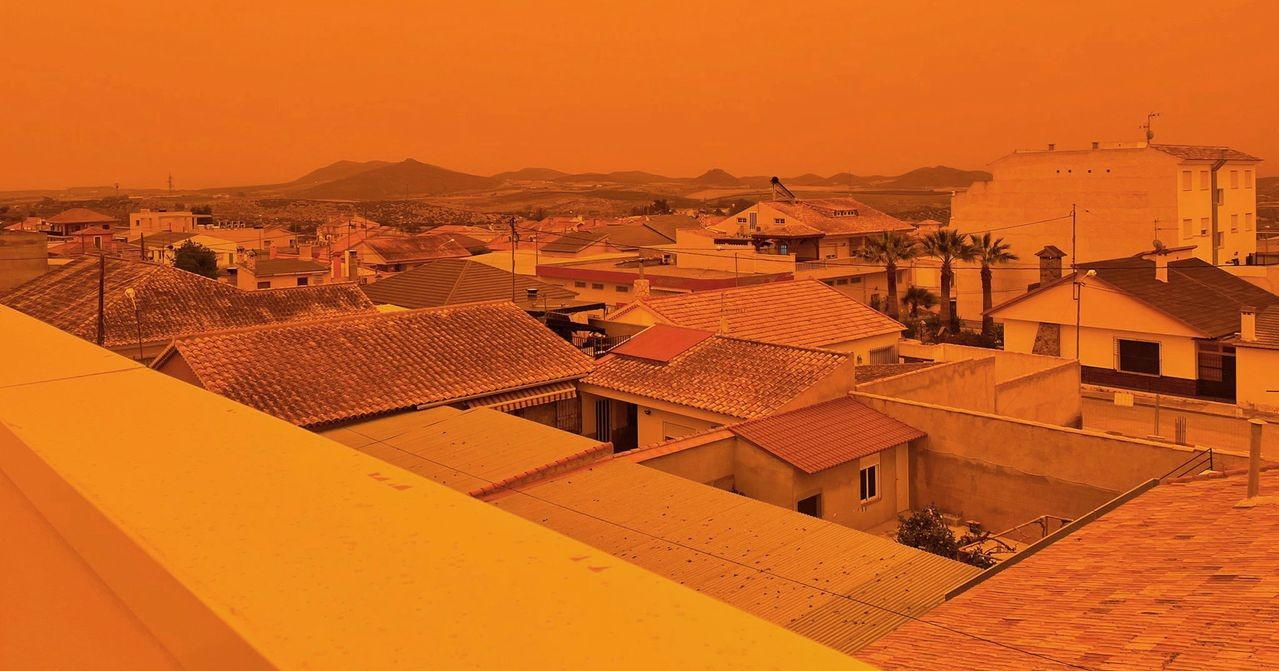
\includegraphics[scale = 0.2]{img/C8/calima.jpg}
    \caption{La calima: un ejemplo del efecto de la componente ambiental}
    \label{fig:calima}
\end{figure}
\newpage
\subsection{Componente difusa}

Cuando la luz impacta sobre un objeto, si este es opaco la luz es reflejada a muchas direcciones, si es translúcido entra en el objeto. Esta componente representa la cantidad de luz que es reflejada. Nosotros consideraremos que la misma cantidad de luz que incide es la que se refleja en todas las direcciones (los objetos son totalmente opacos), y esta depende tanto del ángulo de incidencia como de la normal a la superficie en dicho punto. A esta componente también se le llama reflexión de Lambert por su relación con el modelo de Lambert.

Fijada una fuente de luz, la iluminación difusa $I_d$ se obtiene mediante el producto de la reflectividad difusa del material $k_d\in\R^3$, la intensidad de la luz $I_p$ y el coseno del ángulo que forman la normal al punto ($\vec N$) y la dirección de la fuente de luz ($\vec L_p$), el cual, si $\vec N$ y $\vec L_p$ están normalizados se calcula simplemente como el producto escalar $\vec N\cdot \vec L_p$ (véase imagen \ref{fig:difusa}). Por tanto,
\begin{equation}
    I_{d_p} = I_p k_d (\vec N\cdot \vec L_p)
\end{equation}
La componente difusa final es la suma de las componentes difusas calculadas para cada una de las fuentes de luz.
\begin{equation}
    I_d = \sum_{p=1}^k I_p k_d (\vec N\cdot \vec L_p)
\end{equation}

\begin{figure} [ht]
    \centering
    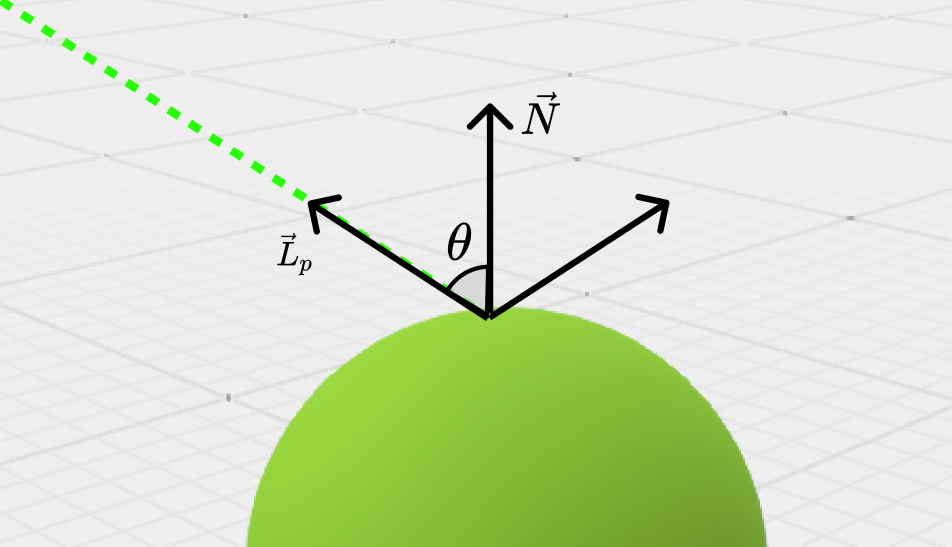
\includegraphics[scale = 0.25]{img/C8/difusa.png}
    \caption{Esquema de los vectores utilizados en la componente difusa}
    \label{fig:difusa}
\end{figure}

Fijémonos que este cálculo es independiente de la posición de la cámara, solo depende de la superficie y la fuente de luz.

\subsection{Componente especular}

Esta componente representa a las reflexiones directas de la fuente de luz sobre un objeto con brillo. Es la intensidad especular mediante la que conseguimos efectos brillantes y metalizados. La percepción de la iluminación especular depende ahora sí de la posición de la cámara respecto a la superficie. Concretamente, fijada una fuente de luz, la componente especular se ve afectada por el ángulo $\alpha$ que forman el vector que une el punto de la superficie que estamos evaluando con el punto de vista, llamémoslo  $\vec V$, y la dirección que tomaría un vector reflejado por la superficie proveniente de la fuente de luz, $\vec R_p$. Véase la imagen \ref{fig:especular} para mayor claridad. El tamaño del resplandor que causan estos brillos se regula con una constante real $n\in\R$ que es parte de las propiedades del material.

\begin{figure} [ht]
    \centering
    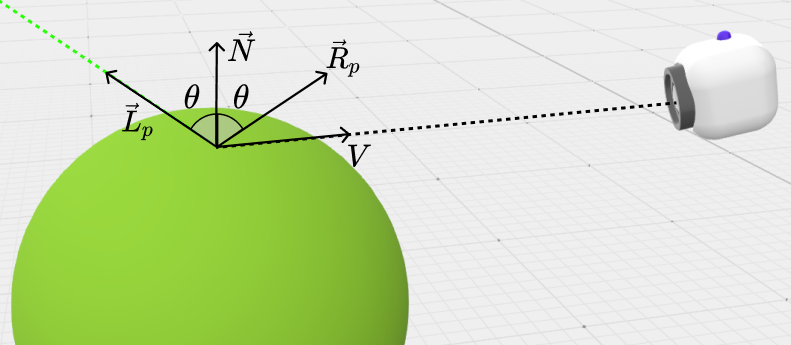
\includegraphics[scale = 0.35]{img/C8/especular.png}
    \caption{Esquema de los vectores utilizados en la componente especular}
    \label{fig:especular}
\end{figure}

A partir de toda esta información, la iluminación especular $I_s$ se calcula con el producto de la reflectividad especular del material $k_s$, la intensidad de la luz $I_p$ y el coseno del ángulo $\alpha$ elevado a $n$. Asumiendo que $\vec R_p$ y $\vec V$ son unitarios, $\cos\alpha=\vec R_p\cdot \vec V$, por lo que tenemos que
\begin{equation}
    I_{s_p} = I_p k_s (\vec R_p\cdot \vec V)^n
\end{equation}   
Al igual que en el caso de la componente difusa, el resultado final es la suma de las componentes especulares generadas por todas las fuentes de luz.
\begin{equation}
    I_s = \sum_{p=1}^k I_p k_s (\vec R_p \cdot \vec V)^n
\end{equation}

\subsection{Sombras arrojadas}
\label{subsection:sombras}

Hay algunas situaciones en las que las que no se aplica iluminación difusa ni especular, y es en el caso de que la luz no incida directamente sobre el punto. En este caso, al no incidir la luz se considera que el punto está en la sombra provocada por dicha luz. Hay varias formas de saber si un punto concreto está o no en la sombra. Pensemos primero en puntos que están `en la cara oculta' de un objeto. Es decir, pertenecen a una zona de un objeto sobre la cual una fuente de luz concreta no incide. Para determinar esto se puede utilizar la normal a la superficie en dicho punto, $\vec N$, y el vector dirección de la fuente de luz, $\vec L_p$. Si el coseno del ángulo $\theta$, que recordemos que es el vector formado por $\vec N$ y $\vec L_p$, es negativo, entonces consideramos que la luz no incide sobre el punto, véase la imagen \ref{fig:excepcion}.

\begin{figure} [ht]
    \centering
    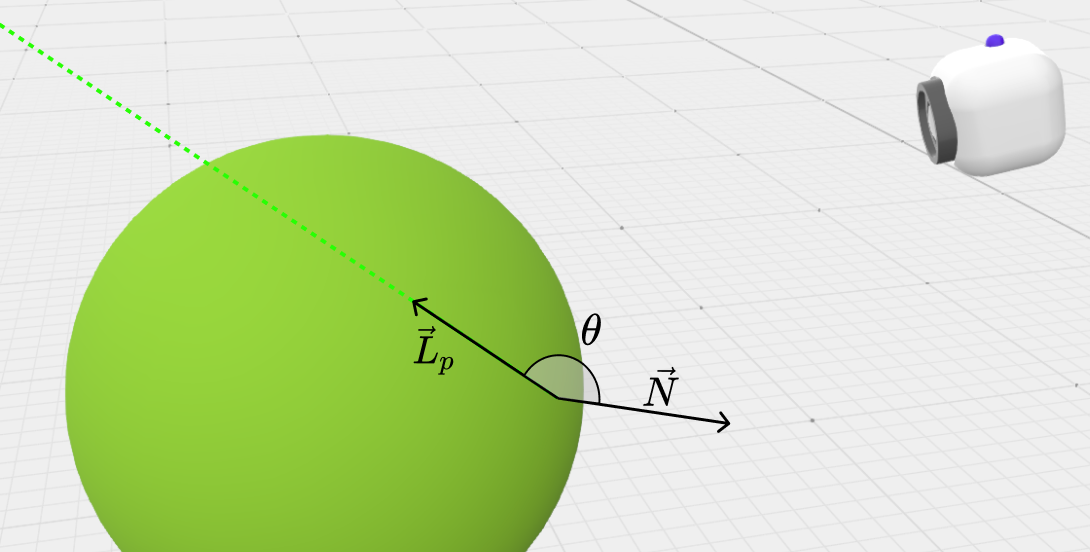
\includegraphics[scale = 0.25]{img/C8/excepcion.png}
    \caption{Punto sobre el que no incide la luz}
    \label{fig:excepcion}
\end{figure}

El problema que esta condición es suficiente únicamente en casos de objetos convexos, como las esferas, ya que si la superficie tiene puntos tapados por el propio objeto el cálculo afirmaría que la luz incide sobre el mismo cuando realmente no es así. Fíjese en el caso del tubo de la figura \ref{fig:no-convexo}.

\begin{figure} [ht]
    \centering
    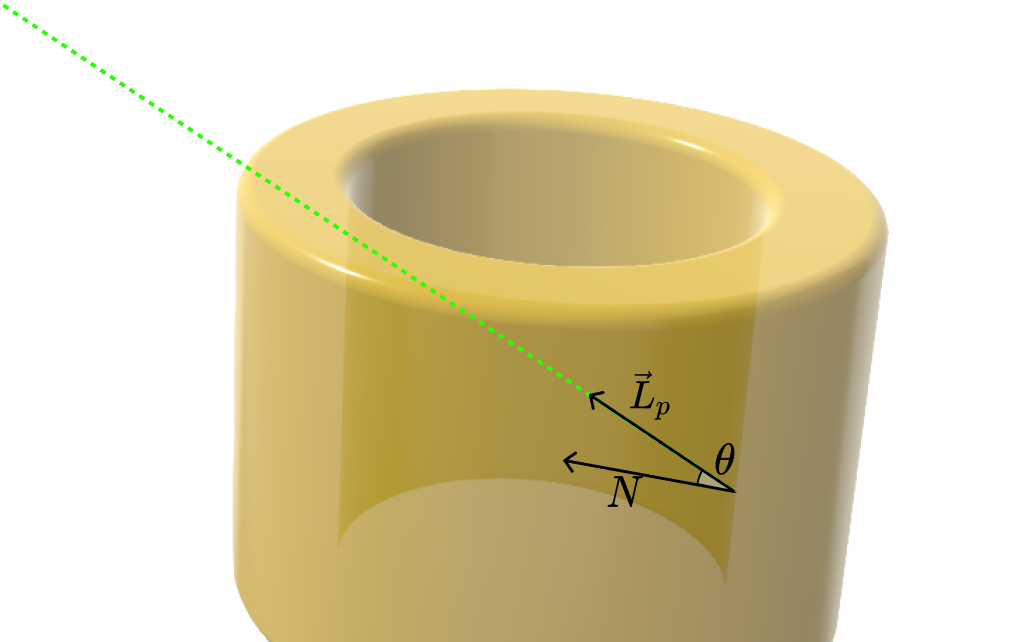
\includegraphics[scale = 0.25]{img/C8/no-convexo.png}
    \caption{Ejemplo de objeto no convexo y punto a la sombra}
    \label{fig:no-convexo}
\end{figure}

En estos casos, la forma de saber si el punto está o no a la sombra es lanzar un rayo en la misma dirección que la luz y averiguar si existe alguna intersección con algún objeto de la escena. En caso de que la haya multiplicamos por $0$ el valor de la componente difusa y la especular (el punto está a la sombra). Si no existe impacto se establece que la luz incide directamente sobre el punto y se multiplicarían por $1$ las componentes difusa y especular. Este proceso debe repetirse con cada una de las fuentes de luz que se utilicen.

Por ejemplo, fíjese en la imagen \ref{fig:sombras}. Si se lanza un rayo desde el punto $p_0$, este no encontrará intersección con ningún objeto, por lo que se considera que la luz incide sobre él. Por su parte, $p_1$ está en la parte del objeto sobre la cual no impacta la luz, y si además lanzamos un rayo en dirección a la fuente de luz intersecaría con la propia esfera. Y finalmente, al lanzar un rayo desde $p_2$ éste interseca con la esfera, por lo que se considera que está a la sombra.

\begin{figure} [ht]
    \centering
    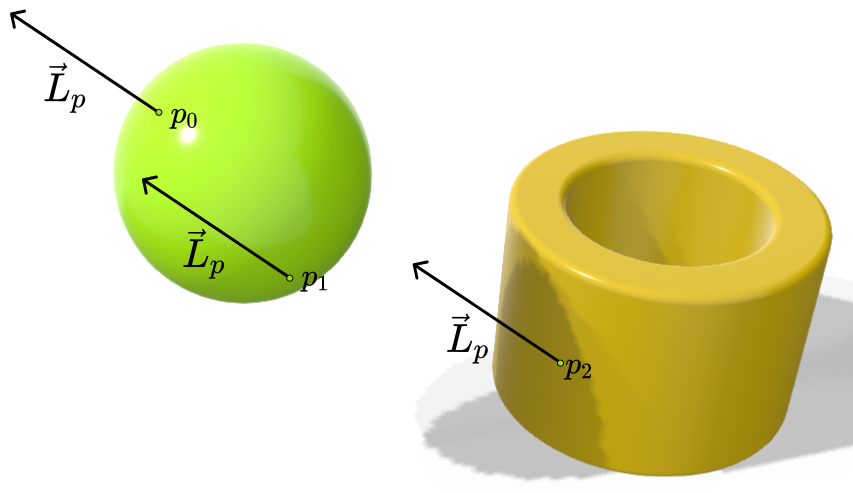
\includegraphics[scale = 0.3]{img/C8/sombras.png}
    \caption{Ejemplos de puntos sobre los que incide y no una fuente de luz}
    \label{fig:sombras}
\end{figure}

Por cualquiera de las dos razones, un punto puede ocurrir que esté a la sombra, en cuyo caso no se calcularían o se anularían las componentes difusa y especular del modelo. Por tanto, las intensidades difusa y especular se redefinen multiplicando cada una de las dos por una constante binaria para cada luz, $c_p$, la cual vale $0$ si el punto evaluado está a la sombra o $1$ si la luz incide sobre el mismo.

\begin{align*}
    I_{d_p} &= c_p I_p k_d (\vec N\cdot \vec L_p)  & I_d &= \sum_{p=1}^k c_p I_p k_d (\vec N\cdot \vec L_p)\\
    I_{s_p} &= c_p I_p k_s (\vec R_p\cdot \vec V)^n & I_s &= \sum_{p=1}^k c_p I_p k_s (\vec R_p \cdot \vec V)^n
\end{align*}

\subsection{Evaluación del modelo de iluminación}

Una vez se han explicado las tres componentes y cómo se calculan podemos evaluar el modelo de iluminación completo sumando las tres componentes.
\begin{equation}
    \label{eq:phong}
    \begin{split}
        I &= I_a + I_d + I_p \\
        &=\frac{1}{k}\sum_{p=1}^k I_p k_a + \sum_{p=1}^{k}c_p I_p k_d (\vec N\cdot \vec L_p) + \sum_{p=1}^{k} c_p  I_p k_s (\vec R_p\cdot \vec V)^n \\
        &=\sum_{p=1}^{k}\left(\frac{1}{k}I_p k_a + c_p I_p k_d (\vec N\cdot \vec L_p) + c_p I_p k_s (\vec R_p\cdot \vec V)^n\right)
    \end{split}
\end{equation}

A modo de adelanto, pero también con el objetivo de aclarar conceptos, obsérvese cómo afecta cada componente del modelo. En las imágenes \ref{fig:componentes-aisladas} vemos el efecto de cada tipo de iluminación por separado. En la imagen (a) observamos en rojo que el efecto de la parte ambiental afecta por igual a todos los puntos, de forma que realmente no da ninguna sensación de volumen. En (b) se puede ver cómo la componente difusa colorea de forma mate en color verde el objeto. Por último, en (c) se observan únicamente brillos especulares azules.

\begin{figure}[ht]
    \centering
    \begin{tabular}{ccc}
      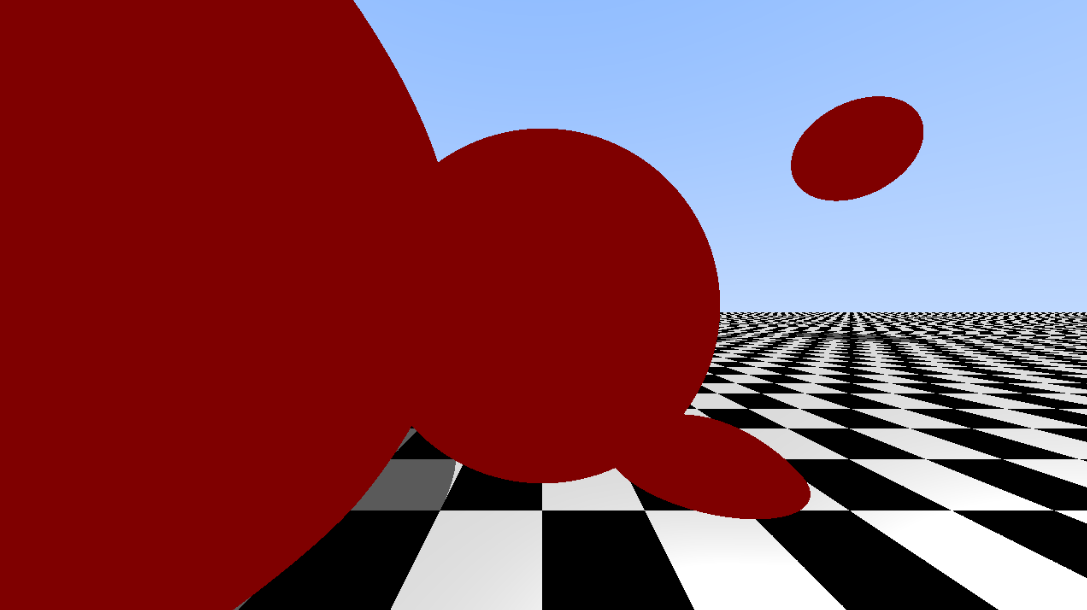
\includegraphics[width=5cm]{img/C8/solo-ambiental.png} &   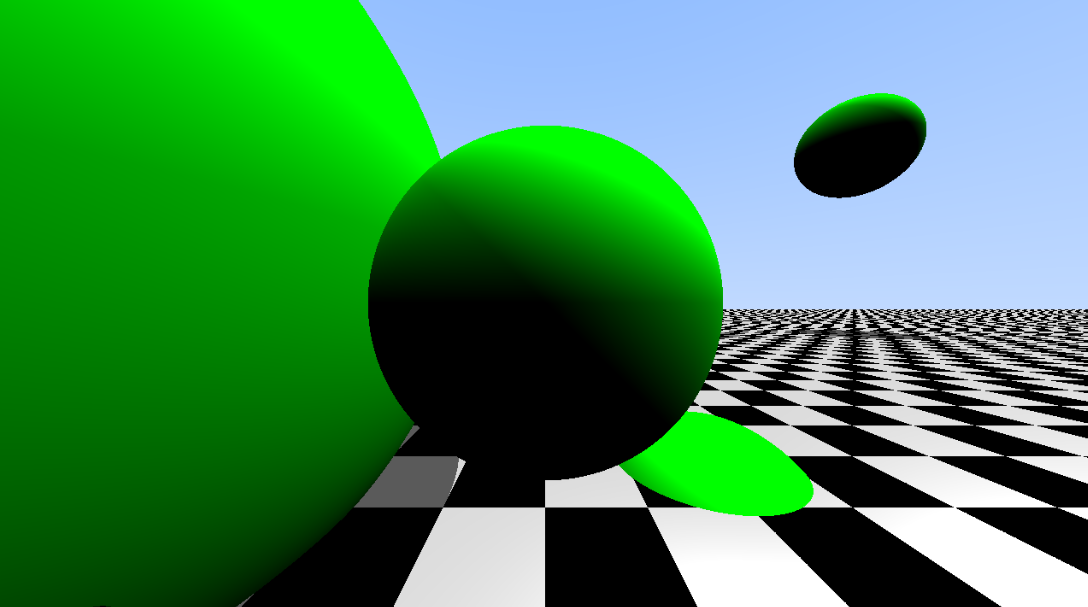
\includegraphics[width=5cm]{img/C8/solo-difusa.png} &   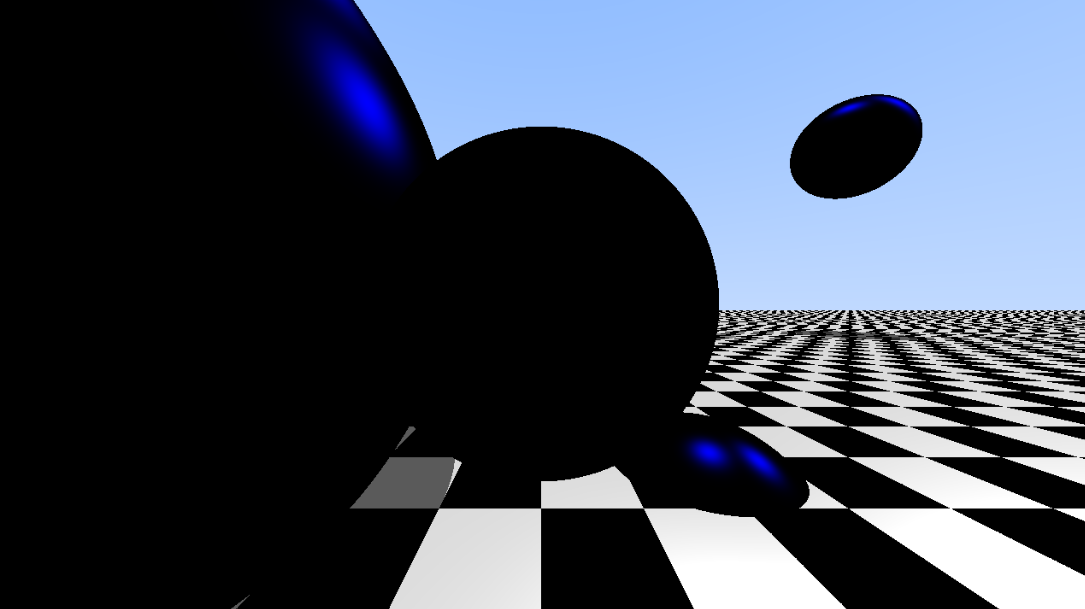
\includegraphics[width=5cm]{img/C8/solo-especular.png} \\
    (a) Ambiental & (b) Difusa & (c) Especular \\[6pt]
    \end{tabular}
    \caption{Componentes aisladas del modelo de Phong}
    \label{fig:componentes-aisladas}
\end{figure}

Y ahora observemos una imagen en la que se aprecian las tres componentes a la vez: la imagen \ref{fig:todas-componentes}. En las esferas predomina el verde, pero se aprecian brillos azules y sombras rojas, pudiendo apreciar perfectamente qué papel desarrolla cada componente del modelo. Fijémonos como efectivamente en los puntos que no incide la luz se ven rojos por el efecto de la componente ambiental.

\begin{figure} [ht]
    \centering
    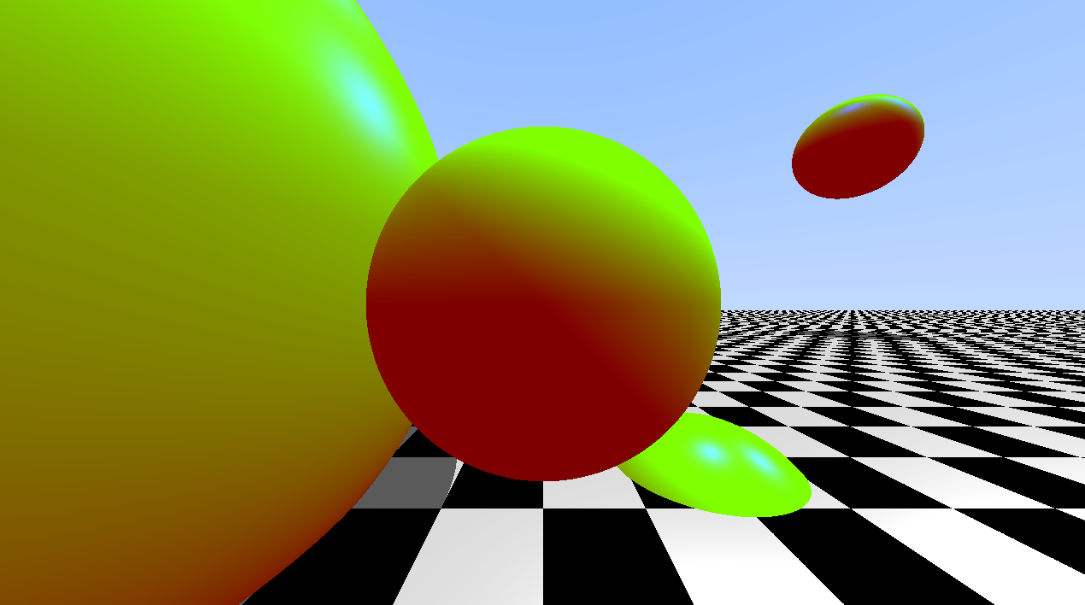
\includegraphics[width=9cm]{img/C8/todas-componentes.png}
    \caption{Acción de todas las componentes}
    \label{fig:todas-componentes}
\end{figure}

\subsection{Implementación del modelo de Phong}

Veamos ahora cómo a partir de la teoría introducida podemos obtener resultados como los de las imágenes \ref{fig:componentes-aisladas} y \ref{fig:todas-componentes}. El elemento básico de un modelo de iluminación es, como no podría ser de otro modo, la fuente de luz. Una fuente de luz ya dijimos que se compone de un vector director y una tripleta RGB que define su intensidad, pero en GLSL los colores vienen representados por 4 componentes, siendo la última la que corresponde a transparencia. Por simplicidad nosotros la consideraremos siempre igual a $1.0$. Por tanto, representamos en GLSL una fuente de luz direccional mediante el siguiente struct.
\begin{lstlisting}
struct Directional_light{
    vec3 dir;   // Direccion de la luz
    vec4 color; // Intensidad RBGA de la luz
};    
\end{lstlisting}

Lo siguiente es fijarnos en que el material del objeto desempeña una labor fundamental, de hecho es el que define finalmente la apariencia del mismo. Este material tiene como elementos las reflectividades ambiental ($k_a$), difusa ($k_d$) y especular ($k_s$), las cuales son también tuplas RGBA. Además de las reflectividades, el exponente de brillo $n$ también es una propiedad del material. De esta forma, podemos representar un material con un struct tal que así:

\begin{lstlisting}
struct Material {
    vec4 ka;    // Reflectividad ambiental
    vec4 kd;    // Reflectividad difusa
    vec4 ks;    // Reflectividad especular
    float sh;   // Exponente de brillo
};
\end{lstlisting}

Como ya hemos comentado, cada objeto tiene un único material, por lo que añadimos a las estructuras \verb|Sphere| y \verb|Plane| un nuevo campo \verb|Material mat;| de forma que a cada esfera y al plano se le puede asignar un material. Además, en caso de intersección almacenábamos información en una estructura \verb|Hit_record|, y esa información es la que nos servía para calcular el color. De igual manera que necesitábamos por ejemplo la normal ahora necesitamos saber el material del objeto con el que impacta el rayo, por lo que añadimos a \verb|Hit_record| también un campo \verb|Material mat;| al cual se le asignaría el material del objeto con el que se produce el choque.

Para calcular la constante $c_p$ con la que conseguir el sombreado necesitamos ahora una función que, dado un punto, trace un rayo en dirección de una fuente de luz dada y devuelva 0 si hay intersección con algún objeto y 1 si no la hay. Fijémonos que debemos calcular intersecciones que estén a una pequeña distancia del punto, ya que en otro caso las funciones que calculan la intersección siempre calcularían que existe impacto (pues el punto que se evalúa está en una superficie), de forma que todos los puntos estarían a la sombra, cosa que no tiene sentido. Además, consideramos que solo las esferas arrojan sombras.

\begin{lstlisting}
float light_is_visible(Directional_light light, vec3 p, 
    Sphere world[ARRAY_TAM], int size) {
    Ray R;
    R.dir = normalize(light.dir);
    R.orig = p;
    float t = 0.01;
    float h;

    return hit_spheres_list(world, size, R, t, MAX_DIST).hit ? 
           0.0 : 1.0; 
}
\end{lstlisting}

Además, con el objetivo de añadir eficiencia e interactividad se ha añadido una variable \verb|uniform| de tipo \verb|bvec3|, es decir, una tripleta de booleanos, que sirve para especificar desde JavaScript qué luces queremos que proyecten sombras. Así podemos proyectar las sombras de la luz que queramos cuando busquemos realismo o desactivarlas cuando queramos mayor rapidez en la ejecución, bajo la limitación de que solo podremos utilizar hasta 3 fuentes de luz.

\begin{lstlisting}
uniform bvec3 u_shadows;
\end{lstlisting}

Con estas variaciones ya podríamos implementar una función que evalúe el modelo de iluminación completo a partir de la ecuación (\ref{eq:phong}). Esta función necesita como argumentos las fuentes de luz, el material, el punto en el que se evalúa el modelo, la normal a la superficie en dicho punto, los objetos que arrojan sombras y el punto $o_c$ desde el que se observa. Toda esta información puede ser recogida en un array de objetos \verb|Directional_light|, en la estructura \verb|Hit_record| que almacena la información del choque, en la variable global \verb|u_lookfrom| y el vector de esferas. Presentamos por tanto el código de dicha función.

\begin{lstlisting}
vec4 evaluate_lighting_model( 
  Directional_light lights[ARRAY_TAM], int num_lights, 
  Hit_record hr,
  Sphere world[ARRAY_TAM], int size ) {
  
  Material mat = hr.mat;
  Directional_light light;
  vec3 light_dir;
  vec3 view_dir = normalize(u_lookfrom - hr.p);
  vec3 normal = normalize(hr.normal);
  vec4 ambient, diffuse, specular;
  float visibility;
  vec4 L_in = vec4(0.0, 0.0, 0.0, 1.0);
  if(num_lights > 0){
    for(int i = 0; i < ARRAY_TAM; i++){
      if(i == num_lights) break;
      ambient = vec4(0.0, 0.0, 0.0, 1.0);
      diffuse = vec4(0.0, 0.0, 0.0, 1.0);
      specular = vec4(0.0, 0.0, 0.0, 1.0);
      light = lights[i];
      ambient += mat.ka*light.color;
      if(num_lights <= 3 && !u_shadows[i]) visibility = 1.0;
      else 
        visibility = light_is_visible(light,hr.p,world,size);
      light_dir = normalize(light.dir);
      float cos_theta = max(0.0,dot(normal,light_dir));
      // Solo si la fuente de luz es visible desde el punto
      if(cos_theta > 0.0 && visibility > 0.0) {
        // Reflection direction
        vec3 reflection_dir = reflect(-light_dir, normal);
        diffuse = mat.kd * cos_theta;
        specular = mat.ks * pow( max(0.0, 
          dot(reflection_dir, view_dir)), 
          mat.sh);
      }
      L_in += visibility * light.color * (diffuse + specular);
    }
  }
  L_in += ambient/float(num_lights);
  return vec4(L_in.xyz, 1.0);
}
\end{lstlisting}

Lo siguiente es editar, aunque muy levemente, las funciones \verb|hit_sphere| y \verb|hit_plane| para que en caso de existir intersección asignen a \verb|result.mat| el material de la esfera \verb|S.mat| y el del plano \verb|P.mat| respectivamente. Por último debemos, una vez más, editar \verb|ray_color| para que acepte como argumento el array de luces y hacer las llamadas correspondientes a la función \verb|evaluate_lighting_model|.

Sin embargo, recordemos que el suelo tenía textura de tablero de ajedrez, por lo que no podemos asignar de manera uniforme un material al plano. Lo que sí podemos es editar los parámetros del material utilizado para el suelo asignando a sus componentes blanco o negro según corresponda, aunque a partir de este momento y por pura estética se utilizará un color gris claro \verb|rgb(178,178,178)| en lugar del blanco.

\begin{lstlisting}
vec4 ray_color(Ray r, Sphere world[ARRAY_TAM], int size, 
    Plane P, Directional_light lights[ARRAY_TAM], 
    int num_lights) {

    // r interseca alguna esfera?
    // ...
    if(hr.hit){
        // ... 
        tmp_color = evaluate_lighting_model(lights, 
            num_lights, hr, world, size);
    }

    // r interseca el plano? 
    // ...
    if(hr.hit){
        // ... 
        if(modulus == 0){
            hr.mat.kd = vec4(0.5, 0.5, 0.5, 1.0);
            hr.mat.ks = vec4(0.5, 0.5, 0.5, 1.0);
            hr.mat.sh = 10.0;
        }
        else
            hr.mat.kd = vec4(0.0,0.0,0.0, 1.0);
        tmp_color = evaluate_lighting_model(lights, 
            num_lights, hr, world, size);
    }
    // ...
}
\end{lstlisting}

Y ya por último tan solo tenemos que inicializar las luces y los materiales. En el caso de las luces, hemos utilizado dos fuentes de luz y hemo añadido dos variables \verb|uniform| para elegir los colores de ambas, aunque inicialmente serán blancas. Las direcciones de estas luces son $(1,1,0)$ y $(0,1,0)$. Respecto a los materiales, el del plano únicamente tiene la componente difusa y especular que se le asigna en \verb|ray_color| y el de las esferas es editable por el usuario, de forma que tenemos 4 variables \verb|uniform| que son editables dinámicamente y a partir de las cuales se inicializa el material de las esferas.

\begin{lstlisting}
// Material parametrizable
uniform vec4 u_ka;
uniform vec4 u_kd;
uniform vec4 u_ks;
uniform float u_sh;

// Colores de las luces
uniform vec4 u_lightColor0;
uniform vec4 u_lightColor1;

// ... 

// Materiales
Material mat, ground_material;
mat.ka = u_ka;
mat.kd = u_kd;
mat.ks = u_ks;
mat.sh = u_sh;

ground_material.ka = vec4(0.0, 0.0, 0.0, 1.0);
ground_material.ks = vec4(0.0, 0.0, 0.0, 1.0);
ground_material.sh = 1.0;

// Esferas
// ... 
S1.mat = mat; S2.mat = mat;
S3.mat = mat; S4.mat = mat;
// ...

// Plano
// ...
P.mat = ground_material;
// ... 

// Luces
Directional_light lights[ARRAY_TAM];
int num_lights = 2;
Directional_light l0, l1;
l0.color = u_lightColor0; 
l1.color = u_lightColor1;
l0.dir = vec3(1.0, 1.0, 0.0);
l1.dir = vec3(0.0, 1.0, 0.0);
lights[0] = l1; lights[1] = l2;
// ... 

gl_FragColor = ray_color(r, world, num_spheres, 
    P, lights, num_lights);
\end{lstlisting}

Evidentemente todos estos parámetros se pueden modificar y poner los que queramos, para finalmente obtener las imágenes y la coloración que deseemos. Como ejemplo, obsérvese el resultado obtenido al modificar algunos de los parámetros en la imagen \ref{fig:phong-final}.

\begin{figure} [ht]
    \centering
    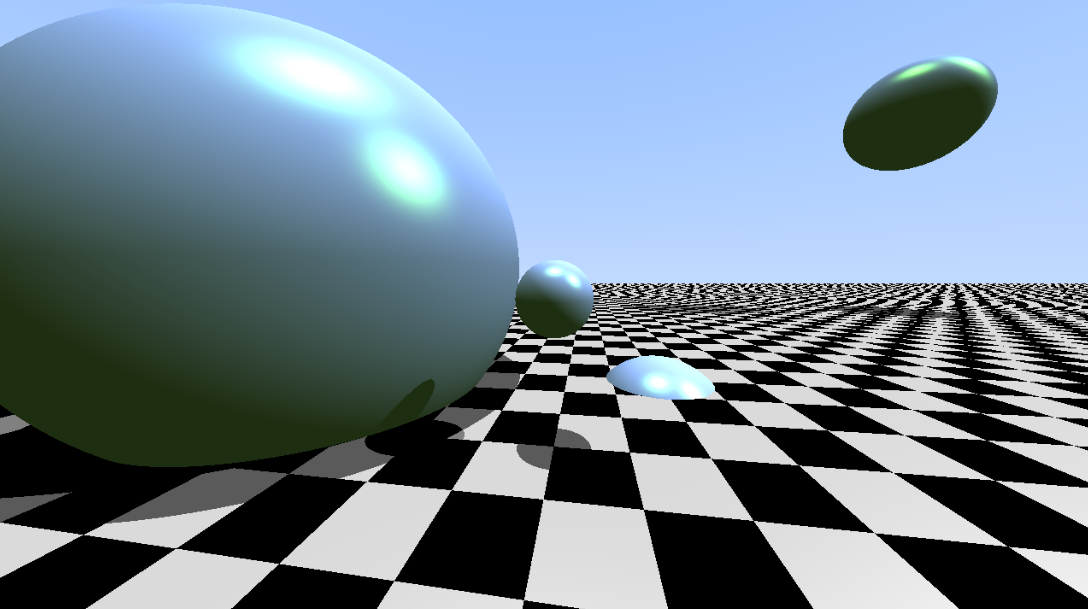
\includegraphics[width=12cm]{img/C8/phong-final.png}
    \caption{Escena aplicando el modelo de Phong completo}
    \label{fig:phong-final}
\end{figure}

\newpage

\section{SSAA en Ray-Tracing}

En el capítulo \ref{chap:fractales-2D}, y concretamente en la sección \ref{section:SSAA-2D} mostramos la posibilidad de utilizar más de un punto del plano por píxel, calcular el color asociado a cada uno y asignar un valor promedio a \verb|gl_FragColor|. Esta modificación producía imágenes y bordes más suavizados, con un nivel más alto de realismo. En 3D, esta técnica es igualmente aplicable y necesaria de hecho, fíjese por ejemplo en la imagen \ref{fig:no-antialiasing-3D}, en la cual se aprecian las irregularidades en los bordes de las fichas negras y blancas y a distancias mayores la textura se distorsiona bastante.

\begin{figure} [ht]
    \centering
    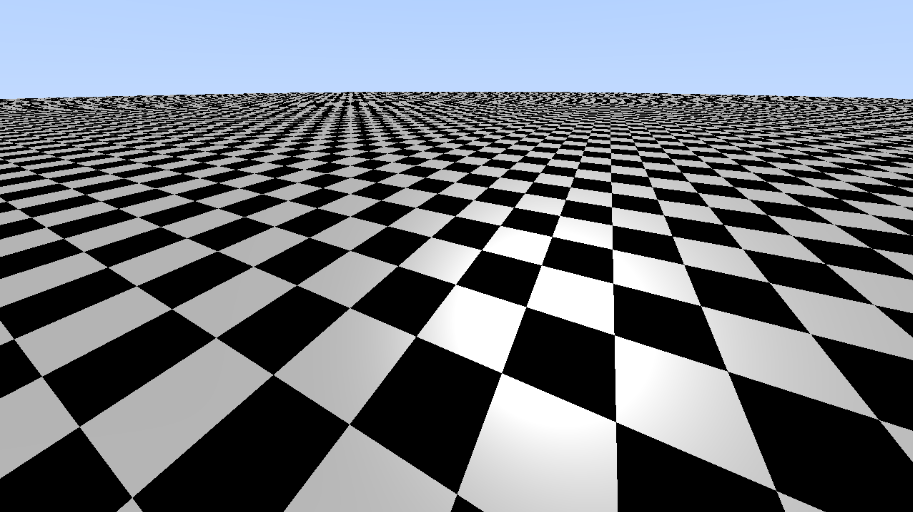
\includegraphics[width=12cm]{img/C8/no-antialiasing.png}
    \caption{Suelo antes de aplicar antialiasing}
    \label{fig:no-antialiasing-3D}
\end{figure}

Por suerte, podemos aplicar SSAA también en 3D. De igual forma que calculamos $n^2$ puntos por píxel en la región del plano que representábamos en 2D, podemos calcular, por cada píxel, $n^2$ puntos del plano de proyección, lanzar un rayo en dirección de cada uno y promediar los colores calculados para cada rayo. La metodología es prácticamente análoga a la utilizada en la sección \ref{section:SSAA-2D}, teniendo en cuenta que en este caso calculamos puntos del plano de proyección para posteriormente crear rayos. De hecho, invitamos al lector que visite dicha sección si no entiende algunos de los razonamientos, los cuales hemos abreviado por su parecido a los ya explicados en la sección \ref{section:SSAA-2D}. Procedemos entonces a explicar la metodología.


En \verb|main|, cuando obtenemos \verb|u,v| y creamos el rayo, ahora debemos calcular $n^2$ coordenadas. Recordemos, de la sección \ref{section:camara}, \verb|u,v| son las coordenadas de dispositivo normalizadas en $[0,1]$, es decir:
\begin{lstlisting}
vec2 uv = (gl_FragCoord.xy + vec2(0.5)) / vec2(nx, ny);
float u = uv.x;
float v = uv.y;
\end{lstlisting}

Si ahora en lugar de utilizar un rayo por píxel que se dirige al centro del mismo deseamos lanzar $n^2$ rayos uniformemente distribuidos por el la superficie del píxel, tenemos que dividir su ancho en $n$ intervalos, análogamente el alto. Por tanto, dividimos cada píxel en una cuadrícula $n\times n$ donde cada fragmento mide $h_w:=\frac{1}{n_x\cdot n}$ en anchura y de $h_h:=\frac{1}{n_y \cdot n}$ en altura. Tras esto, centramos la cuadrícula sumando $\frac{1}{2}h_w$ en ancho y $\frac{1}{2}h_h$ en alto (revisitar imagen \ref{fig:SSAA}).

Seguidamente, calculamos los $n^2$ colores, uno por cada rayo que lancemos. Por cada rayo calculamos la coordenada de dispositivo normalizada del punto hacia el cual queremos lanzar el rayo, llamamos a \verb|get_ray|, a \verb|ray_color| y sumamos el valor de retorno de esta última. Finalmente dividimos esta suma entre $n^2$ para calcular el color promedio y este es el que finalmente asignaríamos a \verb|gl_FragColor|.

Para calcular la coordenada de dispositivo normalizada del punto $i$-ésimo iteramos un índice $i=0,\dots,n^2$, de forma que $i/n$ sería la fila e $i\%n$ la columna. Es decir, a la coordenada de dispositivo normalizada inicial habría que sumarle $(i/n)h_w + \frac{1}{2}h_w$ en anchura e $(i\%n)h_h+ \frac{1}{2}h_h$ en altura para obtener la coordenada normalizada a la que lanzar el rayo. El código GLSL por tanto sería el siguiente

\begin{lstlisting}
// Antialiasing
vec2 uv = (gl_FragCoord.xy) / vec2(nx, ny);
float u = uv.x;
float v = uv.y;

int nSamples = 3; // O cualquier otro numero natural
float hw = 1.0 / (float(nx * nSamples)),
      hh = 1.0 / (float(ny * nSamples));
Ray r;
vec4 sum_colors = vec4(0.0, 0.0, 0.0, 1.0);

for(int i = 0; i < 1000; i++) {
    if(i == nSamples*nSamples) break;
    int x =  i/nSamples;
    int y =  i - nSamples*x;
    u = uv.x + float(x) * hw + 0.5 * hw;
    v = uv.y + float(y) * hh + 0.5 * hh;
    r = get_ray(cam, u, v);
    sum_colors += ray_color(r, world, num_spheres, ground, 
        lights, num_lights);
}

gl_FragColor = sum_colors / float(nSamples*nSamples);
\end{lstlisting}

Con esta modificación y fijando el valor que consideremos en $n$ (\verb|nSamples|) se consiguen resultados como el de la figura \ref{fig:antialiasing-3D}. Como se puede ver, los bordes son más suaves y de mejor calidad y las regiones más lejanas tienen mejor resolución.

\begin{figure} [ht]
    \centering
    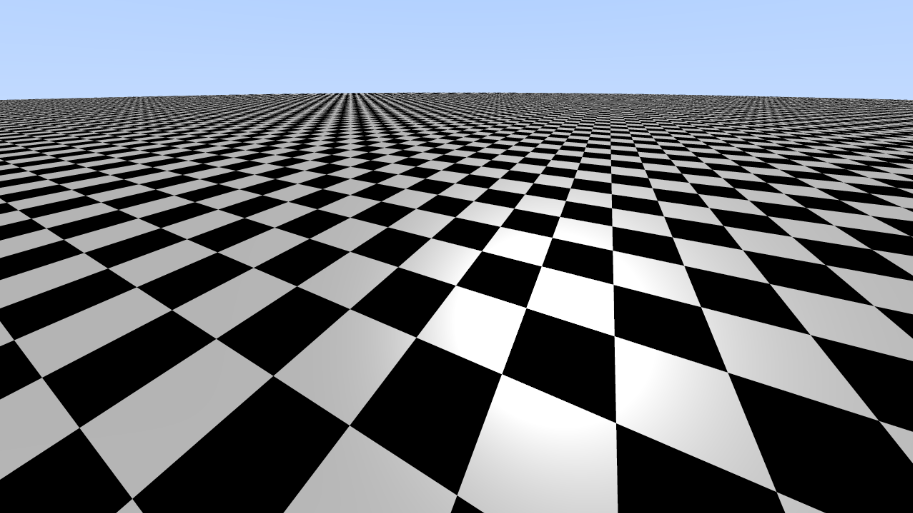
\includegraphics[width=12cm]{img/C8/antialiasing.png}
    \caption{Suelo tras aplicar antialiasing}
    \label{fig:antialiasing-3D}
\end{figure}

De nuevo, por cuestiones de eficiencia e interactividad, se incluye en el software la posibilidad de decidir si se desea o no aplicar SSAA en 3D, y en caso afirmativo, cuántos rayos por píxel se desean trazar. Esto se consigue mediante las variables \verb|uniform| \verb|u_antialiasing| y \verb|u_nSamples|, cuyas funciones son las mismas que las ya explicadas en la sección \ref{section:SSAA-2D}, aunque se puede deducir del código presentado a continuación.

\begin{lstlisting}
uniform bool u_antialiasing;
uniform int u_nSamples;
// ...
void main() {
    // ... 
    if(u_antialiasing) {
        // Aplicar SSAA
        int nSamples = u_nSamples;
        // ... 
    }
    else {
        // No aplicar SSAA
        // ...
    }
}   
\end{lstlisting}

\newpage

Para terminar esta exposición y este capítulo mostraremos una última imagen que resume todo lo desarrollado: Ray-Tracing, intersecciones con distintos cuerpos, posicionamiento de cámara, iluminación, sombras y SSAA.

\begin{figure} [ht]
    \centering
    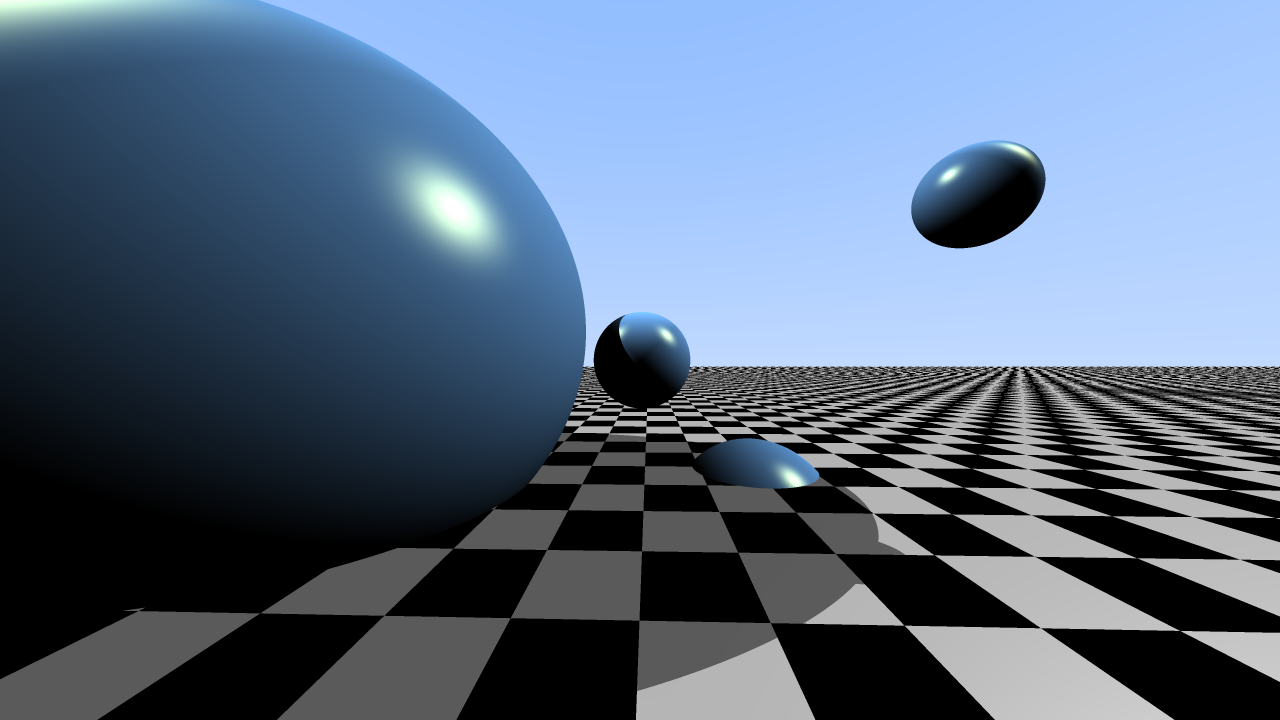
\includegraphics[width=12cm]{img/C8/imagen-final.png}
    \caption{Imagen final del capítulo \ref{chap:ray-tracing}}
    \label{fig:imagen-final}
\end{figure}

